\newif\ifdraft
\draftfalse

% draft mode is true: \drafttrue
%   - uses \documentclass{article} instead of afitThesis.sty
% draft mode is false: \draftfalse
%   - uses afitThesis.sty

\ifdraft
  \documentclass{article}
  \usepackage[letterpaper, margin=.8in]{geometry}
  \usepackage[doi=false,isbn=false,url=false]{biblatex}
  \addbibresource{back/references.bib}
\else
  \documentclass[12pt,letterpaper,oneside]{book}
\fi

%\usepackage{fancyvrb}
\usepackage{physics} 
	% \pdv, \qty

\usepackage{breqn}
	% \begin{dmath} \end{dmath} - produces less vertical space
\usepackage{soul} 
	% \hl{highlighted text}


%\usepackage{float}
%\usepackage{subcaption}
%\captionsetup{compatibility=false}
%\usepackage[justification=centering]{caption}

\ifdraft
  \usepackage{graphicx}
\else
  \usepackage{afitStyleFiles/afitThesis}
  \usepackage{afitStyleFiles/sf298}
  \usepackage{cite}
	% makes references [1-3] instead of [1,2,3]
\fi


\usepackage{dirtytalk} % quotations with \say{}
	
\usepackage{showkeys} % show labels and citations

\usepackage{amsmath} 
	% \begin{multiline} \\ \end{multiline}
	% \begin{cases}

\usepackage[hidelinks]{hyperref}
%\usepackage [autostyle, english = american]{csquotes}
%\MakeOuterQuote{"}
\usepackage[noabbrev, capitalize, nameinlink]{cleveref}
%	- spell out equations, capitalize the first letter,
% 		and make the numbers themselves hyperlinks

\usepackage{float} % Places the figure float at precisely the location in the LaTeX code

%\usepackage{subfigure}
% for plots
\usepackage{subcaption}
%
\usepackage[justification=centering]{caption}

\graphicspath{{figures/}}
% define custom commands
%\newcommand{\regmark}{\raisebox{5pt}{\tiny \circledR}\xspace}
%\newcommand{\trademark}{\raisebox{5pt}{\tiny TM}\xspace}
%\newcommand{\mca}{\texttt{Mathematica}\regmark}
%\newcommand{\Latex}{\LaTeX\xspace}

\newcommand*{\tensor}[1]{\overline{\overline{#1}}}
\newcommand*{\pO}{\partial\Omega}
\newcommand*{\dO}{\, d\Omega}
\newcommand*{\dS}{\, dS}
\newcommand*{\plus}{\texttt{+}}
\newcommand*{\minus}{\texttt{-}}
%\def\plus{\texttt{+}}
%\def\minus{\texttt{-}}
\newcommand*{\sfrac}[2]{\textstyle\frac{#1}{#2}}
	% style for superscript fractions
\newcommand*{\mdot}{\dot{m}}
\newcommand*{\trm}[1]{\textrm{#1}}
	% style for regular text in math mode

\newcommand*{\Qs}{Q_{\textrm{sonic}}}
	% Q_sonic

\DeclareMathAlphabet{\mathpzc}{OT1}{pzc}{m}{it} % for curly math

% Create a new theorem style called a Corollary.
% If you don't have any, then just comment this out.
%\theoremstyle{plain} % Default
%\newtheorem{cor}{Corollary}[chapter]

%Custom Commands for Student

\newcommand{\primerAddress}{{L:$\backslash$Courses$\backslash$PHYS$\backslash$LaTeX}\xspace}

% ----------------------------------------- CREF Package
\creflabelformat{equation}{#2\textup{#1}#3}
\newcommand{\crefrangeconjunction}{\,-}
	% make cross-references conjoined by -

% --- unused
%\newcommand{\crefrangeconjunction}{\,\minus}
%\crefname{equation}{equation}{equations}
%\Crefname{equation}{Equation}{Equations}% For beginning \Cref
%\crefrangelabelformat{equation}{(#3#1#4--#5#2#6)}

%\crefdefaultlabelformat{#2#1#3}

%\crefmultiformat{equation}{equations (#2#1#3}{, #2#1#3)}{#2#1#3}{#2#1#3}
%\Crefmultiformat{equation}{Equations (#2#1#3}{, #2#1#3)}{#2#1#3}{#2#1#3}


\ifdraft
	% abbreviationFull[shock-wave/boundary layer interaction]{SWBLI}
	\newcommand*{\abbreviationFull}[2]{#1 (#2)}

	% \symbol[density]{$\rho$}
	\renewcommand{\symbol}[2]{#2}
    
    % makes chapter titles cool
    \usepackage{titlesec}
    \titleformat{\chapter}[display]{}			{\filleft\scshape\chaptername\enspace\thechapter}{-2pt}{\filright \Huge \bfseries}[\vskip4.5pt\titlerule]
 \titleformat{name=\chapter, numberless}[block]{}{}{0pt}{\filright \Huge \bfseries}[\vskip4.5pt\titlerule]

 \titlespacing{\chapter}{0pt}{-15pt}{25.5pt}
 \titlespacing{name=\chapter, numberless}{0pt}{16pt}{15pt}
 
 
    %\titleformat
	%{\chapter} % command
	%[display] % shape
	%{\bfseries\Large\itshape} % format
	%{Chapter \thechapter} % label
	%{0.5ex} % sep
	%{
    %	\rule{\textwidth}{1pt}
    %	\vspace{1ex}
    %	\centering
	%} % before-code
	%[
	%	\vspace{-0.5ex}%
	%	\rule{\textwidth}{0.3pt}
	%] % after-code
    
    
\else
\fi








\begin{document}

\ifdraft
	\author{Dayle}
	\title{DRAFT}
	\maketitle
    \tableofcontents
\else
	\frontmatter
    \title{DRAFT}
    \tableofcontents
    \listoffigures
    \mainmatter
\fi

\pagebreak
% - - - - - - - - - - - - - - - - - - - - - - - - - - - - - - - - - - - -

% ====================================================== Introduction
	\chapter{Introduction} \label{introduction}
\section{Motivation}

Shock waves are a natural phenomenon that arise in many supersonic applications. When the shock interacts with the boundary layer, the situation becomes complex and is an important design consideration for a large number of applications in transonic and supersonic flows. This interaction occurs so pervasively that it has been termed the \abbreviationFull[shock-wave/boundary layer interaction]{SWBLI}. Successful applications of aircraft, missiles, inlets, or wind tunnel designs in supersonic flow is contingent on the favorable behavior of the SWBLI in both internal and external flows \cite{Gaitonde2013}. Three key issues that arise due to SWBLI are identified by Holden: peak heating, dynamic loads, and effects of separated unsteady flows \cite{Holden1986}. These three issues and their effects on practical applications are discussed in greater depth below followed by concluding remarks summarizing the motivation and objectives of this research.

%SWBLI is an important design factor for a large number of applications in transonic and supersonic flows. These interactions, however weak or strong, occur so ubiquitously that consideration must be given for successful application of any kind of transonic or supersonic application, whether the flow is internal or external and regardless of the body in quesiton, whether aircraft, missiles, rockets, and projectives. The SWBLI affects or determines the maximum, mean, and fluctuating pressure levels on a body, which in turn affect the local stresses on the body, heat flux, and flow structure which can have the same impacts on other body surfaces, though the overall energy levels are not affected very much. \cite{Gaitonde2013}

% (peak heating in three-dimensional turbulent interactions, dynamic loads generated in transitional regions of SWBLI, effects of the unsteadiness of separated flows, etc.) are as relevant today as research topics as they were 14 years ago. \cite{Dolling2001}]'

% - - - - - - - - - - - - - - - - - - - - - - - - - - - - - - - - - - - - - - - - - - - - - 
\subsection{Peak Heating}
The severe effects of peak heating is well documented in SWBLI, particularly in hypersonic flows. Peak rates vary between 10 to 100 times the incoming boundary-layer flow and many times the equivalent stagnation point value \cite{Dolling2001}. Knight and Degrez note that \enquote{heat transfer distribution predictions are generally poor, except for weak interactions, and significant differences are evident between turbulence models... of up to 100\% between experiment and numerical results} \cite{Knight1998}. These high temperatures cause localized stresses which affect the design of practical applications such as geometry, fatigue, material selection, and thermal protection \cite{Dolling2001}.

% - - - - - - - - - - - - - - - - - - - - - - - - - - - - - - - - - - - - - - - - - - - - - 
\subsection{Dynamic Loads}
In many aeronautical applications, parameters of critical importance are imposed by unsteady conditions that can occur during flight, rather than steady conditions. Although these events are rare or do not contribute much to the local average energy, they can correspond to high local stress, which can affect the whole behavior of the system. In supersonic flows, an important case occurs when unsteadiness involves shock waves producing locally large pressure fluctuations. They may act as strong aerodynamic loads and are felt along the whole flow downstream of the shock wave. This occurs in shock-induced separation, where low-frequency unsteadiness is produced \cite{Piponniau2009}.

An example of this is in the controls response system of aircraft and missile bodies. High-speed anti-armor, kinetic energy penetrators (Mach 4-8 at sea level) are configurations of interest to the U.S. Army that pose many simulation and experimental challenges due to the SWBLI. Following discharge from the gun, lateral thrusters or control surfaces may be used to guide and control such projectiles. Accurate characterization of the three-dimensional, unsteady, laminar, transitional, and turbulent interactions that sweep rapidly across is very important and will call for accurate modeling of SWBLI \cite{Dolling2001}. %\hl{also, hypersonics vehicles}

Another example is in plume-induced boundary-layer separation in missile design. The boundary layer separates on the afterbody of the missile rather than at the base itself, a result of the strong adverse pressure gradient generated by the interaction of the expanding plume and surrounding freestream ultimately creating large, unsteady, asymmetric loads on the body itself. The control surfaces and response system must have adequate control authority and response timing to overcome the unsteady loads \cite{Dolling2001}. In the worst case, the control surfaces themselves may experience premature boundary layer separation, causing a total loss of control effectiveness. In both cases, an understanding of the fundamental flow physics allows for missile designs to successfully demonstrate control authority during flight and exhibit maximum performance. Shaw et al. notes that this plume-induced separation feature is not unlike the SWBLI behavior on a compression ramp and share many common features, which can be used to help characterize the separation feature for missile applications \cite{Shaw1998}.

% - - - - - - - - - - - - - - - - - - - - - - - - - - - - - - - - - - - - - - - - - - - - - 
\subsection{Unsteady Flow}
Mixed compression inlets are designed to produce a shock train structure and terminal shock that allows for the highest total pressure recovery required for mixed compression inlets. However, these shocks are sensitive to flow disturbances and flow unsteadiness due to their interaction with the boundary layer. If the effects of unsteady flow are not mitigated, changes to the flow structure can displace the shock wave into a less efficient configuration. If the disturbances are large enough, the terminal shock may move upstream and ultimately out of the inlet, resulting in unstart that produces large transient forces on the airframe and cause engine surge \cite{Dolling2001}. % and ram/scramjet engines

Bleed holes are used as a method of active flow control to mitigate flow unsteadiness inside the inlet. % for both of these neutrally stable phenomenons (terminal shock and shock wave patterns). %\hl{insert compression figure}. 
By adjusting the mass-flow rate reaching the diffuser in response to perturbations in the engine operation or inlet flow, the shock train is stabilized. The disadvantage of such a method is that weight, energy, and thrust is reduced. Factors such as bleed hole location, hole geometry, suction massflow rate, and many others make this an area of ongoing research \cite{Dolling2001}.

% - - - - - - - - - - - - - - - - - - - - - - - - - - - - - - - - - - - - - - - - - - - - - 
\subsection{Current Views}
% B
SWBLI is recognized as a long-standing research area in the aerospace community, garnering wide attention both nationally and internationally \cite{Gaitonde2013}.

A 1996 NASA research announcement stated that \enquote{improved air-breathing engines will require a clearer understanding of the basic flow physics of propulsion system components.} The design of higher performance inlets and nozzles that are \enquote{quieter, shorter, lighter} requires \enquote{benchmark quality data for flowfields including shocks, boundary layers, boundary layer control, separation, heat transfer, surface cooling and jet mixing.} These areas all involve SWBLI in one form or another \cite{Dolling2001}.

The NASA \abbreviationFull[Small Business Innovation Research]{SBIR} solicitation in 2015 emphasized the need for basic research to be relevant for practical applications: \enquote{One of the greatest issues that NASA faces in transitioning advanced technologies into future aeronautics systems is the gap... between the maturity level of technologies developed through fundamental research and the maturity required for technologies to be infused into future air vehicles and operational systems} \cite{NASA2015}. The application of SWBLI research face difficulties on both fronts. On the fundamental research side, \enquote{inadequacies in our understanding of boundary layer turbulence increase reliance upon a more qualitative, physics-guided approach to discovery} \cite{NASA2008} whereas the application of SWBLI research \enquote{concepts for active and passive control of aeroacoustic noise sources... including adaptive flow control technologies, and noise control technology and methods that are enabled by advanced aircraft configurations, including integrated airframe-propulsion control methodologies} \cite{NASA2015}.

%\cite{Schmisseur2013}
%NASA continues to state in its \abbreviationFull[Small Business Innovation Research]{SBIR}
The \abbreviationFull[National Hypersonics Foundational Research Plan]{NHFSP} was developed by \abbreviationFull[Air Force Office of Scientific Research]{AFOSR}, \abbreviationFull[National Aeronautics and Space Administration]{NASA} and Sandia National Laboratory. This plan provides a framework of the main areas in hypersonics research of which SWBLI is a key component. The \abbreviationFull[Research and Technology Office, Air Vehicle Technology]{RTO/AVT} has been an integral part of that development under \abbreviationFull[North Atlantic Treaty Organization]{NATO} \cite{Schmisseur2013}.

Flow control for SWBLI remains a key issue for future technology vehicles but regarded as a complicated and vexing problem. To make the proper trade-offs in design, a deep, physical understanding of the mechanisms of these interactions must be understood with both experimental and computational tools that are both robust and accurate \cite{Dolling2001}.

% ---------------------------------------------------------------------------------
\section{Research Objectives} 

The advancement of \abbreviationFull[Computational Fluid Dynamics]{CFD} and its success shows promise as a critical tool in understanding SWBLI \cite{Zha1998, Dolling2001}. The objective of this research is to use CFD to demonstrate the effect of bleed holes on shock unsteadiness. This research will build further on canonical configurations such as ramps, swept-ramps, and fins by using a forward-facing step and determining if this configuration can be a successful model for mitigating shock unsteadiness.

This research will focus on characterizing the flow physics of a single bleed hole on a flat plate, characterizing the shock unsteadiness of a forward-facing step without active flow control, and observing the effects of bleed holes on the unsteady shock motion.

\Cref{introduction} introduced the subject, motivation, and objectives of this research. 
Chapter II%\Cref{background and theory} 
presents further background information on aerodynamics to include relevant research areas. In addition, it will provide fundamental theory for expected flow phenomena. 
Chapter III explains the computational methodologies used to characterize the computational setup including grid generation, flow solver parameters, turbulence modeling, and the overall experimentation approach. 
Chapter IV presents the results of the grid topology screening, time step/grid refinement study and aerodynamic characterization of the shock unsteadiness at supersonic conditions. The results will be analyzed and compared to experimental data and empirical models. A summary of the research along with conclusions and recommendations for future work are given in Chapter V.

% ---------------------------------------------------------------------------------
%NASA SBIR 2015 Phase I Solicitation
%A1 Air Vehicle Technology

% Inadequacies in our understanding of boundary layer turbulence increase reliance upon a more % qualitative, physics- guided approach to discovery. 
% 
% Concepts for active and passive control of aeroacoustic noise sources for conventional and % advanced aircraft configurations, including adaptive flow control technologies, and noise control % technology and methods that are enabled by advanced aircraft configurations, including integrated % airframe-propulsion control methodologies. 
% 
% 
% NASA SBIR 2015 Phase I Solicitation
% A2 Integrated Flight Systems
% 
% One of the greatest issues that NASA faces in transitioning advanced technologies into future % aeronautics systems is the gap caused by the difference between the maturity level of technologies % developed through fundamental research and the maturity required for technologies to be infused % into future air vehicles and operational systems.
% 
% NASA SBIR 2008 Phase I Solicitation
% A2 Fundamental Aeronautics
% 
% 
% Concepts for active and passive control of aero-acoustic noise sources for conventional and % advanced air- craft configurations, including adaptive flow control technologies, smart structures % for nozzles and inlets, and noise control technology and methods that are enabled by advanced % aircraft configurations, including advanced integrated airframe-propulsion control methodologies;
% 
% 
% This subtopic seeks innovative physics-based models and novel aerodynamic concepts, with an emphasis on flow control, applicable in part or over the entire speed regime from subsonic through hypersonic flight.



%Active flow control concepts targeted at separation control and/or viscous drag reduction with an %emphasis on the development of novel, practical, lightweight, low-energy actuators;
%
%Innovative methods to validate both flow models and aerodynamic concepts with an emphasis on aft-shock effects which are hindered by conventional wind tunnel model mounting approaches;


%B
%To limit these issues, configurations are over-designed with mitigation techniques active, passive, or both to increase control of the SWBLI, which quickly translate to detrimental effects on other important design parameters such as cost, development time, and weight, depending on the application. This directly contradicts the current aeronautical design trends such as commercial transport aircraft that aim to operate at increasingly higher efficiencies. SWBLI pose many challenges in supersonic flight, an area dominated by shock/boundary-layer interactions \cite{Dolling2001}.

% Harloff1996, Syberg1973, Schoenenberger1999, Saunders2014, Paynter1992} 
% Willis1995, Slater2009
% Papadakis2006, Orkwis2013, Oorebeek2012, Duncan2016
% 
% CFD
% duncan
% choe
% 
% Hamed1995
% Hamed2008
% 
% Experimental single hole
% davis
% orkwis
% *papadakis
% schoeneberger
% 
% eichorn2013
% 
% Experimental mult hole
% oorebeek
% paynter
% *saunders
% syberg
% willis
% 
% 
% CFD / mult hole
% harloff
% baurle
% slater



%\subsection{Abstract}


% ====================================================== Background and Theory
	\chapter{Background and Theory} \label{background}
	
%derivations of the navier-stokes equation
\section{Derivation of the Navier-Stokes Equations}

The Navier-Stokes equations describe the motion of viscous fluids and are useful because they describe the physics of scientific and engineering interests. They are used to model the weather, ocean currents, water flow in a pipe, and air flow around a wing. Before deriving the Navier-Stokes equations, assumptions about the flow are made and physical principles are discussed to arrive at the governing equations of fluid dynamics in the following sections.

The first assumption is that the density of the fluid is assumed to be high enough such that the flow is approximated as a continuum. This implies that an infinitesimally small, or differential, element of the fluid still contains a sufficient number of particles for which the mean velocity and mean kinetic energy can be specified. This assumption enables important quantities such as velocity, pressure, temperature, and density to be defined at each point in the fluid. In mathematical terms, the continuum assumption states the mean free path of molecules $\lambda$ is proportionally much smaller than the characteristic length of interest $L$ as shown below
%
$$ k_n = \frac{\lambda}{L} \ll 1 $$
%
where $k_n$ is the Knudsen number. The derivation of the Navier-Stokes equations is based on the fact that the dynamic behavior of the fluid is determined by the following conservation laws:
%
\begin{itemize}
\item Conservation of Mass
\item Conservation of Momentum
\item Conservation of Energy
\end{itemize}

The conservation of these flow quantities means that its total variation inside an arbitrary volume can be expressed as the net effect of the flux, or the rate a flow quantity crosses a boundary surface, any internal forces and sources, and external forces acting on the volume. The flux is decomposed into two parts: one due to convective transport and the other due to molecular motion present in the fluid at rest, or diffusion \cite{BlazekText}. In the following discussion, the finite control volume is defined and a mathematical description of its physical properties for fluid flow is detailed.

% ======================================================= Control Volume
\subsection{Conservation Law within a Control Volume}

A control volume $\Omega$ is defined as an arbitrary and finite region of fluid flow fixed in space and bounded by the closed surface $d\Omega$. The surface element $dS$ represents a small and finite portion of the surface $d\Omega$ and $\vec{n}$ is the associated outward pointing unit normal vector. The net change of a fluid property within the control volume is determined by performing a balance between the net flow in and out of the control volume, such as the force or total energy exchange. This is expressed in a mathematical sense: the change of a given property in time is described as the sum of convective fluxes, diffusive fluxes, volume sources, and surface sources in and through a control volume. This conservation law is shown for the general property $U$ in integral form as shown below:
%
$$ \pdv{t}\int\limits_{\Omega}{U \dO} = \oint\limits_{\pO}{\qty[\kappa\rho\qty(\gradient U^* \cdot \vec{n}) - U\qty(\vec{v}\cdot\vec{n})]\dS} + \int\limits_\Omega{S_v\dO} + \oint\limits_\pO{\qty(\vec{S}_s\cdot \vec{n})\dS} $$

If $U$ is not a scalar but instead a vector $\vec{U}$, the conservation law still holds and is further generalized in vector form as
%
\begin{equation} \pdv{t}\int\limits_\Omega{\vec{U} \dO} = \oint\limits_{\pO}{\qty[\qty(\tensor{F}_d - \tensor{F}_c)\cdot\vec{n}]\dS} + \int\limits_\Omega{\vec{S}_v\dO} + \oint\limits_\dO{\qty(\tensor{S}_s\cdot\vec{n})\dS} \label{eq:conservation} \end{equation}

\noindent
where $\tensor{F}_d$ is the diffusive flux tensor, $\tensor{F}_c$ is the convective flux tensor, $\vec{S}_v$ is the volume source vector, and $\tensor{S}_s$ is the surface source tensor. This formulation of conservation is the basis of the derivation for the conservation laws of mass, momentum, and energy in the continuing discussion.

% ======================================================= Conservation of Mass
\subsection{Conservation of Mass}

The law of conservation of mass states that mass can neither be created nor destroyed. Therefore, the time rate of change of mass within a given control volume is dependent only on the net mass coming in and out of the control volume due to convection. Simply put, convection is the only mechanism by which mass can change within a control volume. The diffusive flux, surface source, and volume source terms all go to zero as a result. This concept is expressed mathematically below:
%
\begin{equation} \pdv{t} \int\limits_{\Omega}{\rho \, d\Omega} + \oint\limits_{\partial \Omega}{\rho\qty(\vec{v}\cdot\vec{n})\,dS} = 0 \label{eq:mass} \end{equation}

\noindent
This yields the conservative, integral form of the continuity equation.

% ======================================================= Conservation of Momentum
\subsection{Conservation of Momentum}

The law of conservation of momentum states that the time rate of change of momentum is equal to the net force acting on a control volume. The momentum of an infinitesimally small portion of the control volume $\Omega$ is $\rho \vec{v}\dO$, where $\vec{v} = \qty[u,v,w]^T$ in a three component Cartesian coordinate system. The variation in time of momentum within the control volume is described as
%
$$ \pdv{t}\int_\Omega{\rho\vec{v}\dO} $$

The convective flux term is the transfer of momentum across the boundary of the control volume
%
$$ -\oint\limits_\pO{\rho\vec{v}\qty(\vec{v}\cdot\vec{n})\dS} $$

The diffusive flux term is zero since there is no diffusion of momentum for a fluid at rest.
The volume sources for momentum conservation are called body forces and described as forces which act directly on the mass of the volume such as gravitational, buoyancy, Coriolis, centrifugal, or electromagnetic forces. They are ignored in this derivation by setting the sources equal to zero.

The surface sources for momentum conservation act directly on the surface of the control volume and consist of two components: the pressure distribution imposed by the fluid surrounding the volume, $-p\tensor{I}$, and the shear and normal stresses resulting from the friction between the fluid and the surface of the volume, $\tensor{\tau}$, as shown below
%
$$ \tensor{S}_s = -p\tensor{I} + \tensor{\tau} $$

\noindent
where $\tensor{I}$ is the unit tensor and $\tensor{\tau}$ is the viscous stress tensor. Each of the terms are summed up in the following mathematical expression: 
%
\begin{equation} \pdv{t}\int\limits_\Omega{\rho\vec{v} \dO} + \oint\limits_\pO{\rho\vec{v}\qty(\vec{v}\cdot\vec{n})\dS} + \oint\limits_\pO{p\vec{n}\dS} - \oint\limits_\pO{\qty(\tensor{\tau}\cdot\vec{n})\dS} = 0 \label{eq:momentum} \end{equation}

\noindent
This yields the conservative, integral form of the momentum equation.

% ======================================================= Conservation of Energy
\subsection{Conservation of Energy}

The law of conservation of energy states that the internal energy of the control volume is equal to the rate of work performed on the volume and the net heat supplied to the volume. The conserved quantity is the total energy per unit volume $\rho E$ and its variation in time within the volume $\Omega$ is expressed as
%
$$ \pdv{t}\int\limits_\Omega{\rho E \dO} $$

Just like the previous mass and momentum equations, the convective flux term is specified as 
%
$$ - \oint\limits_\pO{\rho E \qty(\vec{v}\cdot\vec{n})\dS} $$

In contrast to the previous mass and momentum equations, the diffusive flux term is present in the energy equation and describes the diffusion of heat due to molecular thermal conduction. The diffusive flux term $\vec{F}_d$ is written in the form of Fourier's law of heat conduction, which characterizes heat diffusion as the heat transfer due to temperature gradients
%
$$ \vec{F}_d = -k\grad T $$

\noindent
where $k$ is the thermal conductivity coefficient and $T$ is the absolute static temperature.

The volume source for the energy equation is the volumetric heating due to the absorption or emission of radiation, or due to chemical reactions as well as work done by the body forces. These volume sources are ignored and not considered for this derivation.

The surface source term is the time rate of work done by pressure and the shear and normal stresses on the fluid element
%
$$ \vec{S}_s = - p\vec{v} + \tensor{\tau}\cdot\vec{v} $$

\noindent
where $\tensor{\tau}$  is the stress tensor
%
\begin{equation}
  \tensor{\tau} =
  \begin{bmatrix}
    \tau_{xx} & \tau_{xy} & \tau_{xz} \\
    \tau_{yx} & \tau_{yy} & \tau_{yz} \\
    \tau_{zx} & \tau_{zy} & \tau_{zz}
  \end{bmatrix} \label{eq:stress_tensor}
\end{equation} 

The off-diagonal elements of $\tensor{\tau}$ represent the viscous shear stresses and defined as
%
\begin{align} \begin{split}
  \tau_{xy} &= \tau_{yx} = \mu\qty(\pdv{u}{y} + \pdv{v}{x}) \\
  \tau_{xz} &= \tau_{zx} = \mu\qty(\pdv{u}{z} + \pdv{w}{x}) \\
  \tau_{yz} &= \tau_{zy} = \mu\qty(\pdv{v}{z} + \pdv{w}{y})
  %\label{hi}
\end{split} \label{eq:visc_shear_stresses} \end{align}

The diagonal elements represent the viscous normal stresses and defined as
%
\begin{align} \begin{split}
  \tau_{xx} &= \lambda\qty(\pdv{u}{x}+\pdv{v}{y}+\pdv{w}{z}) + 2\mu\pdv{u}{x} \\
  \tau_{yy} &= \lambda\qty(\pdv{u}{x}+\pdv{v}{y}+\pdv{w}{z}) + 2\mu\pdv{v}{y} \\
  \tau_{zz} &= \lambda\qty(\pdv{u}{x}+\pdv{v}{y}+\pdv{w}{z}) + 2\mu\pdv{w}{z} 
\end{split} \label{eq:expanded_visc_norm}\end{align}

\noindent
where $\lambda$ represents the second viscosity and $\mu$ represents the dynamic viscosity. Stoke's hypothesis eliminates $\lambda$ by relating the second viscosity and the dynamic viscosity as a bulk viscosity, which represents the property that is responsible for energy dissipation in a fluid of uniform temperature during a change in volume at a finite rate as shown.
%
\begin{equation} \lambda + \frac{2}{3}\mu = 0 \label{eq:stokes} \end{equation}

\noindent
The diagonal elements are then simplified using Stoke's hypothesis (\cref{eq:stokes}) for the viscous normal stresses (\cref{eq:expanded_visc_norm}) as shown below
%
\begin{align} \begin{split}
  \tau_{xx} &= 2\mu\Bigg[\pdv{u}{x} - \frac{1}{3}\qty(\pdv{u}{x}+\pdv{v}{y}+\pdv{w}{z})\Bigg] \\
  \tau_{yy} &= 2\mu\Bigg[\pdv{u}{x} - \frac{1}{3}\qty(\pdv{u}{x}+\pdv{v}{y}+\pdv{w}{z})\Bigg] \\
  \tau_{zz} &= 2\mu\Bigg[\pdv{u}{x} - \frac{1}{3}\qty(\pdv{u}{x}+\pdv{v}{y}+\pdv{w}{z})\Bigg]
  %
\end{split} \label{eq:visc_norm_stresses} \end{align}
%\end{align}

%\begin{align} \begin{split}
%  \tau_{xy} &= \tau_{yx} = \mu\qty(\pdv{u}{y} + \pdv{v}{x}) \\
%  \tau_{xz} &= \tau_{zx} = \mu\qty(\pdv{u}{z} + \pdv{w}{x}) \\
%  \tau_{yz} &= \tau_{zy} = \mu\qty(\pdv{v}{z} + \pdv{w}{y})
%  %\label{hi}
%\end{split} \label{eq:visc_norm_stresses} \end{align}


\noindent
The terms are summed in the following mathematical expression:
%
\begin{equation} \begin{split} \pdv{t}\int\limits_\Omega{\rho E \dO} + \oint\limits_\pO{\rho E\qty(\vec{v}\cdot\vec{n})\dS} &= \oint\limits_\pO{k\qty(\grad T\cdot\vec{n})\dS} - \oint\limits_\pO{p\qty(\vec{v}\cdot\vec{n})\dS} \\ & \quad + \oint\limits_\pO{\qty(\tensor{\tau}\cdot\vec{v})\cdot\vec{n}\dS} \end{split} \label{eq:energy} \end{equation}
%
This yields the conservative, integral form of the energy equation.

% ======================================================= Closing the Equations
\subsection{Closing the Equations}

The mass, momentum, and energy equations are collectively referred to as the Navier-Stokes equations, representing a system of five equations in three dimensions for the five conserved variables $\rho$, $\rho u$, $\rho v$, $\rho w$, and $\rho E$. However, the governing equations contain nine unknown flow field variables: \symbol[density]{$\rho$}, \symbol[x-component of velocity]{$u$}, \symbol[y-component of velocity]{$v$}, \symbol[z-component of velocity]{$w$}, \symbol[internal energy (double-check)]{$E$}, \symbol[pressure]{$p$}, \symbol[temperature]{$T$}, $\mu$, and $k$. Therefore, four additional equations are needed to close the equations, which is accomplished by formulating thermodynamic relations between the two unknown state variables for pressure, $p$, and temperature, $T$. For an ideal perfect gas, the equation of state assumes the form
%
\begin{equation} p = \rho R T \label{eqn:eqn_of_state} \end{equation}

\noindent
where $R$ denotes the specific molecular gas constant. This equation can be written as a function of the conserved variables by using the definition of enthalpy
%
\begin{equation} H = h + \frac{\qty|\vec{v}|^2}{2} = E + \frac{p}{\rho} \label{eqn:enthalpy} \end{equation}

\noindent
which relates the total enthalpy to the total energy. Using the definitions
%
$$ R = c_p - c_v, \qquad \gamma = \frac{c_p}{c_v}, \qquad h = c_p T $$
%
the enthalpy equation (\cref{eqn:enthalpy}) is substituted into the equation of state (\cref{eqn:eqn_of_state}) to obtain for the pressure as a function of the conserved variables
%
$$ p = \qty(\gamma - 1) \rho \qty[E - \frac{u^2+v^2+w^2}{2}] $$

Calculating temperature becomes trivial with the aid of \cref{eqn:eqn_of_state}. Dynamic viscosity $\mu$ is strongly dependent on temperature but only weakly dependent on pressure. Sutherland's formula describes this relationship for air (in SI units)
%
$$ \mu = \frac{1.45 T^{\frac{3}{2}}}{T+110} \cdot 10^{\minus 6} $$

\noindent
where the temperature, $T$, is in degrees Kelvin ($K$). %Thus, at $T = 288 $K one obtains $\mu = 1.73 \cdot 10^{\minus 5} $ kg/ms. 
The Prandtl number ($Pr$) is a dimensionless number defined as the ratio of momentum diffusivity to thermal diffusivity
%
$$ Pr = \dfrac{c_p \mu}{k} $$

The Prandtl number is assumed constant in the flow for air with a value of $P_r = 0.72$. Therefore, the thermal conductivity $k$ is determined from temperature. \cite{BertinText,TannehillText,BlazekText,TuText,WhiteText}.


% ======================================================= Finite Volume
\subsection{Integral Form of the Navier-Stokes Equations}

For the complete system of the Navier-Stokes equations, \cref{eq:mass,eq:momentum,eq:energy} are combined using the general conservation law (\cref{eq:conservation}) into the following vectorized form:
%
\begin{equation} \pdv{t} \int\limits_\Omega \vec{Q} \dO + \oint\limits_{\dO}(\vec{F_c}-\vec{F_v}) \dS = 0 \label{eq:iNS} \end{equation}

\noindent
where $\vec{Q}$ is the vector of conserved variables in three dimensions, $\vec{F}_c$ represents the convective fluxes, and $\vec{F}_d$ represents the diffusive fluxes. Note that \cref{eq:iNS} does not include any source terms. These three vectors for the five total equations are defined as follows
%
\begin{equation}
\vec{Q} = \begin{bmatrix} \rho \\
  \rho u \\
  \rho v \\
  \rho w \\
  \rho E \end{bmatrix} \label{eq:iQ}
\end{equation}
%
\begin{equation}
\vec{F}_c = \begin{bmatrix} \rho V \\
  \rho uV + n_x p \\
  \rho vV + n_y p \\
  \rho wV + n_z p \\
  \rho HV \end{bmatrix} \label{eq:iFc}
\end{equation}
%
\begin{equation}
\vec{F}_v = \begin{bmatrix} 0 \\
  n_x\tau_{xx} + n_y\tau_{xy} + n_z\tau_{xz} \\
  n_x\tau_{yx} + n_y\tau_{yy} + n_z\tau_{yz} \\
  n_x\tau_{zx} + n_y\tau_{zy} + n_z\tau_{zz} \\
  n_x\Theta_x + n_y\Theta_y + n_z\Theta_z \end{bmatrix} \label{eq:iFv}
\end{equation}

% \noindent
% \begin{align} 
% \vec{Q} &= \begin{bmatrix} \rho \\
%   \rho u \\
%   \rho v \\
%   \rho w \\
%   \rho E \end{bmatrix} \label{eq:q} \\
% %\vec{S} &= \begin{bmatrix} 0 \\
% %  \rho f_{e,x} \\
% %  \rho f_{e,y} \\
% %  \rho f_{e,z} \\
% %  \rho \vec{f}_e \cdot \vec{v} + \dot{q}_h \end{bmatrix} \label{eq:s} \\
% \vec{F}_c &= \begin{bmatrix} \rho V \\
%   \rho uV + n_x p \\
%   \rho vV + n_y p \\
%   \rho wV + n_z p \\
%   \rho HV \end{bmatrix} \label{eq:fc} \\
% \vec{F}_v &= \begin{bmatrix} 0 \\
%   n_x\tau_{xx} + n_y\tau_{xy} + n_z\tau_{xz} \\
%   n_x\tau_{yx} + n_y\tau_{yy} + n_z\tau_{yz} \\
%   n_x\tau_{zx} + n_y\tau_{zy} + n_z\tau_{zz} \\
%   n_x\Theta_x + n_y\Theta_y + n_z\Theta_z \end{bmatrix} \label{eq:fv}
% \end{align}

\noindent
where $V$ is the contravariant velocity 
%
\begin{equation} V \equiv \vec{v} \cdot \vec{n} = n_x u + n_y v + n_z w \label{eq:contravariant_vel} \end{equation}

\noindent
and where 
%
\begin{align} \begin{split}
  \Theta_x = u\tau_{xx} + v\tau_{xy} + w\tau_{xz} + k\pdv{T}{x} \\
  \Theta_y = u\tau_{yx} + v\tau_{yy} + w\tau_{yz} + k\pdv{T}{y} \\
  \Theta_z = u\tau_{zx} + v\tau_{zy} + w\tau_{zz} + k\pdv{T}{z} 
\end{split} \label{eq:theta} \end{align}

\cref{eq:iNS,eq:iQ,eq:iFc,eq:iFv,eq:contravariant_vel,eq:theta} ultimately describe the exchange of mass, momentum, and energy through the boundary $\dO$ of a fixed control volume $\Omega$ in what is known as the integral form of the Navier-Stokes equations.

% ======================================================= Differential Form
\subsection{Differential Form of the Navier-Stokes Equations}

Though not always the case, the integral form of the Navier-Stokes equations is better understood in the context of the finite volume method. However, the code used in this research (OVERFLOW) uses the finite-difference method and so the differential form of the Navier-Stokes equations is presented for completeness.

Recall the integral form of the Navier-Stokes equations were presented in the discussion from the starting assumption that the control volume was fixed in space, an Eulerian frame of reference. An alternative approach examines the differential element moving with the fluid flow, a Lagrangian frame of reference, rather than a control volume fixed in space. The two frames of reference are related through the Reynolds transport theorem which relates the rate of change of a system property within a fixed region (control volume) to the time derivative of a system property (differential element). Applying the theorem to the integral form of the governing equations (\cref{eq:iNS}) leads to the differential form as shown below
%
$$ \pdv{}{t}\int\limits_\Omega{\vec{Q}\dO} + \int\limits_\Omega{\gradient \cdot\qty(\vec{F}_c - \vec{F}_v)\dO} = 0 $$

The integral drops out for an arbitrary control volume $\Omega$ and the equation is written in the differential form as 
%
$$ \pdv{\vec{Q}}{t} + \gradient\cdot \qty(\tensor{F}_c - \tensor{F}_v) = 0 $$

It is typical to combine the convective and viscous fluxes and expand the gradient operator $\gradient$ to arrive at the generalized form
%
\begin{equation} 
\pdv{\vec{Q}}{t} + \pdv{\vec{E}}{x} + \pdv{\vec{F}}{y} + \pdv{\vec{G}}{z} = 0 
\label{eq:dNS}
\end{equation}
%
%where $\vec{E}$ represents the fluxes in the $x$-direction, $\vec{F}$ represents the flux
%
where $\vec{E}$, $\vec{F}$, and $\vec{G}$ represent the fluxes in the $x$-, $y$-, and $z$-directions, respectively, as shown below

\begin{equation}
\vec{Q} = \begin{bmatrix} \rho \\
  \rho u \\
  \rho v \\
  \rho w \\
  \rho E \end{bmatrix} \label{eq:dQ}
\end{equation}
%
\begin{equation}
\vec{E} = \begin{bmatrix} \rho u \\
  \rho u^2 + p - \tau_{xx} \\
  \rho uv - \tau_{xy} \\
  \rho uw - \tau_{xz} \\
  (\rho E + p)u - \Theta_x \end{bmatrix} \label{eq:dE}
\end{equation}
%
\begin{equation}
\vec{F} = \begin{bmatrix} \rho v \\
  \rho uv - \tau_{xy} \\
  \rho v^2 + p - \tau_{yy} \\
  \rho vw - \tau_{yz} \\
  (\rho E + p)v - \Theta_y \end{bmatrix} \label{eq:dF}
\end{equation}
%
\begin{equation}
\vec{G} = \begin{bmatrix} \rho w \\
  \rho uw - \tau_{xz} \\
  \rho vw - \tau_{yz} \\
  \rho w^2 + p - \tau_{zz} \\
  (\rho E + p)w - \Theta_z \end{bmatrix} \label{eq:dG}
\end{equation}
%
\cref{eq:theta,eq:dNS,eq:dQ,eq:dE,eq:dF,eq:dG} describe the change in mass, momentum, and energy at an infinitesimally small element of the flow in what is known as the differential form of the Navier-Stokes equations. 

%so something something something \cite{Orkwis2013, Syberg1973, Paynter1993} %









	%derivations of the navier-stokes equation
\section{Boundary Conditions}

The Navier-Stokes equations are a set of partial differential equations (PDEs) for which an analytical solution does not currently exist, but can be solved approximately and iteratively using computers. In computing solutions to PDEs, the appropriate application of boundary conditions is a key ingredient in arriving at a unique and practical solution. The two most common boundary conditions as it pertains to the Navier-Stokes equations are the Dirichlet boundary condition, where the value of the function is specified on the boundary, and the Neumann boundary condition, where the normal derivative of the function is specified on the boundary. 

The Dirichlet boundary condition is applied in the supersonic inflow, supersonic outflow, periodic, and specified pressure conditions where the values at the boundary are prescribed. Both the Dirichlet and Neumann boundary conditions are applied in the no-slip wall condition. The boundary conditions are enforced for higher-order methods by dummy nodes, artificial nodes surrounding the computational domain whose field values are set to expand the stencil. A simple overview of the no-slip wall, supersonic inflow, supersonic outflow, periodic, and specified pressure boundary conditions are presented in the following discussion.

% ======================================================= No-Slip Wall
\subsection{No-Slip Wall}

The interaction between molecules of a viscous fluid and a solid surface create a condition where the fluid velocity is zero relative to the boundary, hence the name \enquote{no-slip} wall. The assumption that there is no heat transfer through the wall is additionally employed to determine the other conserved variables at the boundary
%
%\begin{equation}
%\frac{\partial T}{\partial n}|_{\textrm{wall}} =  0
%\end{equation}
%
%Thus, the conserved variables at the boundary are
%
\begin{equation}
\vec{Q}_b = \begin{bmatrix} \rho_i \\
  0 \\
  0 \\
  0 \\
  \qty(\rho E)_i \end{bmatrix}
\end{equation}
%
where the subscript $i$ denotes the value one node interior from the boundary and the subscript $b$ denotes the value at the node on the boundary. For implementations of higher-order methods at the boundary, the dummy node is prescribed values such that the fluxes, both convective and viscous, are zero through the boundary.
%
\begin{equation}
\vec{Q}_d = \begin{bmatrix} \rho_i \\
  -(\rho u)_i \\
  -(\rho v)_i \\
  -(\rho w)_i \\
  \qty(\rho E)_i \end{bmatrix}
\end{equation}
%
where the subscript $d$ denotes the value at the dummy node, or one node exterior from the boundary.

% ======================================================= Inflow
\subsection{Supersonic Inflow}

Consider a supersonic flow and the type of domain boundary that is present at the inflow. If one examines the direction of signal propagation for this condition, the characteristics carry information from the exterior of the domain toward the interior in all cases. This indicates that all the information at the inflow boundary for a supersonic flow must be specified using the freestream conditions so that information will always be carried toward the boundary from the exterior. Thus the conserved variables at the boundary are
%
\begin{equation}
\vec{Q}_b = \begin{bmatrix} \rho_\infty \\
  (\rho u)_\infty \\
  (\rho v)_\infty \\
  (\rho w)_\infty \\
  \qty(\rho E)_\infty \end{bmatrix}
\end{equation}
%
where the subscript $\infty$ denotes freestream values. The dummy nodes are likewise prescribed the same interior values so that freestream values are propagated into the domain
%
\begin{equation}
\vec{Q}_g = \begin{bmatrix} \rho_\infty \\
  (\rho u)_\infty \\
  (\rho v)_\infty \\
  (\rho w)_\infty \\
  \qty(\rho E)_\infty \end{bmatrix}
\end{equation}

% ======================================================= Extrapolate
\subsection{Supersonic Outflow}

The numerical implementation of the supersonic outflow boundary condition must prevent any outgoing disturbances from reflecting back into the flow field. At the outflow boundaries, the characteristics all carry the same sign for the supersonic case and the solution must be determined entirely from conditions based on the interior. Thus, the flow properties at the boundary are prescribed values one node interior from the boundary
%
\begin{equation}
\vec{Q}_b = \begin{bmatrix} \rho_i \\
  (\rho u)_i \\
  (\rho v)_i \\
  (\rho w)_i \\
  \qty(\rho E)_i \end{bmatrix}
\end{equation}
%

The dummy nodes are likewise prescribed the same interior values so that no information propagates into the domain

\begin{equation}
\vec{Q}_g = \begin{bmatrix} \rho_i \\
  (\rho u)_i \\
  (\rho v)_i \\
  (\rho w)_i \\
  \qty(\rho E)_i \end{bmatrix}
\end{equation}

% ======================================================= Specified Pressure
\subsection{Specified Pressure Outflow}

The specified pressure outflow boundary condition is useful to simulate discharge of flow into an ambient pressure such as a plenum, ambient air, or a vacuum. The implementation requires density and the three velocity components to be extrapolated from the interior of the physical domain to the boundary. Since the pressure is specified, the fifth conserved variable, energy, is determined from the equation of state (\cref{eqn:eqn_of_state}) as shown below%
%
\begin{equation}
\vec{Q}_b = \begin{bmatrix} \rho_i + \qty(p_b-p_i)/c_0^2 \\
  \rho_u \qty[u_d + n_x\qty(p_i-p_b)/\qty(\rho_0 c_0)] \\
  \rho_v \qty[v_d + n_y\qty(p_i-p_b)/\qty(\rho_0 c_0)] \\
  \rho_w \qty[w_d + n_z\qty(p_i-p_b)/\qty(\rho_0 c_0)] \\
  p_b/\qty(\gamma-1) + \rho\qty(u^2 + v^2 + w^2)/2 \end{bmatrix}
\end{equation}
%
where $p_b$ is the specified pressure at the boundary. Field values for the dummy node is obtained by linear extrapolation from the states $i$ and $b$.

% ======================================================= Specified Pressure
\subsection{Periodic}

There are certain practical applications where the flow field is periodic with respect to one or multiple coordinate directions. In such a case, it is sufficient to simulate the flow within one of the repeating regions. The correct interaction with the remaining physical domain is enforced with a periodic boundary condition. The boundary condition is typically applied to two identical planes that are not collocated in space and is denoted below with the superscripts $1$ and $2$
%
\begin{equation}
\vec{Q}_b^1 = \begin{bmatrix} \rho_i^2 \\
  (\rho u)_i^2 \\
  (\rho v)_i^2 \\
  (\rho w)_i^2 \\
  \qty(\rho E)_i^2 \end{bmatrix} \qquad \qquad 
\vec{Q}_b^2 = \begin{bmatrix} \rho_i^1 \\
  (\rho u)_i^1 \\
  (\rho v)_i^1 \\
  (\rho w)_i^1 \\
  \qty(\rho E)_i^1 \end{bmatrix}
\end{equation}
%

The dummy nodes follow the same principle and are prescribed values one node further into the domain, denoted by the subscript $i+1$ as shown
%
\begin{equation}
\vec{Q}_d^1 = \begin{bmatrix} \rho_{i+1}^2 \\
  (\rho u)_{i+1}^2 \\
  (\rho v)_{i+1}^2 \\
  (\rho w)_{i+1}^2 \\
  \qty(\rho E)_{i+1}^2 \end{bmatrix} \qquad \qquad 
\vec{Q}_d^2 = \begin{bmatrix} \rho_{i+1}^1 \\
  (\rho u)_{i+1}^1 \\
  (\rho v)_{i+1}^1 \\
  (\rho w)_{i+1}^1 \\
  \qty(\rho E)_{i+1}^1 \end{bmatrix}
\end{equation}




	\section{Turbulence Modeling}
% ======================================================= Turbulence Modeling
%\subsection{Turbulence Modeling}

The Navier-Stokes equations as described thus far hold only for laminar flow. However, it is known from simple observation of fluid flow that small disturbances in laminar flow can cause the flow to transition to turbulence. The onset of this chaotic and random state of motion found in turbulent flows depends on the ratio of inertial to viscous forces, or Reynolds number. At low Reynolds numbers, viscous forces dominate, the naturally occurring disturbances dissipate away, and the flow remains laminar. At high Reynolds numbers, the inertial forces are sufficiently large to amplify the disturbances and transition from laminar to turbulent flow occurs.

Fundamentally, turbulence is a continuum phenomenon since the smallest scales of turbulence are very large compared to the molecular scales. This implies the Navier-Stokes equations are of deterministic nature since it contains all of the physics of turbulent fluid motion \cite{BlazekText} but the direct simulation of turbulent flows presents a significant problem. Despite the performance of modern supercomputers, a direct numerical simulation of turbulence (DNS) by the time-dependent Navier-Stokes equations is applicable only to relatively simple flow problems at low Reynolds numbers in the order of $10^4 \minus 10^5$. The simulation must resolve a wide range of scales from the largest, energy bearing eddies to the smallest, vorticity containing eddies that accomplish the continuous dissipation of mechanical energy into internal energy. An accurate turbulent simulation must capture the entire range of active scales - a range that increases rapidly as Reynolds number increases. Widespread utilization of DNS is prevented by the fact that the number of grid points needed for sufficient spatial resolution scales as $Re^2$ and the CPU-time as $Re^3$. Therefore, the effects of turbulence must be accounted for in an approximate matter and a large variety of turbulence models were developed for this purpose.

%The origins of turbulence modeling find their roots with fluid mechanics pioneers such as Prandtl, Taylor, von Karman, and Kolmogorov. Their work was characterized by simplicity combined with physical insight, where their models introduced the minimum amount of complexity while capturing the essence of the relevant physics. This philosophy is the basis for good turbulence models 
The Reynolds-Averaged Navier-Stokes equations is outlined and two models of turbulence and a hybrid model are discussed in the following section. 

% ======================================================= RANS
\subsection{Reynolds-Averaged Navier-Stokes Equations}

In the late 1800s, Reynolds modified the governing equations by decomposing the flow variables into a mean and fluctuating component to describe the flow field \cite{Reynolds1903}. For example, velocity $u$ is decomposed into a time-averaged component, $\bar{u}_i$, and a fluctuating component, $u_i^\prime$. Recall the momentum equation in three-dimensional, differential form from \cref{eq:dNS}:
%
$$ \rho \pdv{u_i}{t} + \rho u_j \pdv{u_i}{x_j} + \pdv{p}{x_i} - \pdv{\tau_{ij}}{x_j} = 0 $$

where $\tau_{ij}$ is the stress tensor described in compact tensor notation, succinctly capturing \cref{eq:visc_shear_stresses,eq:visc_norm_stresses} as
%
$$ \tau_{ij} = \mu \qty(\pdv{u_i}{x_j} + \pdv{u_j}{x_i}) - \qty(\frac{2\mu}{3})\pdv{u_k}{x_k}\delta_{ij} $$
%
where $\delta_{ij}$ represents a $\medmuskip=0mu 3\times3$ identity matrix. After careful treatment of averaged correlated products, the Reynolds-averaged momentum equation is
%
%$$ \rho \pdv{\bar{u}_i}{t} + \rho \bar{u}_j \pdv{\bar{u}_i}{x_j} + \pdv{\bar{p}}{x_i} - \pdv{}{x_j}\Bigg[\mu\qty(\pdv{\bar{u}_i}{x_j} + \pdv{\bar{u}_j}{x_i}) - \rho \overline{u_i^'u_j^'}\Bigg] = 0 $$
%
\begin{equation} \rho \pdv{\bar{u}_i}{t} + \rho \bar{u}_j \pdv{\bar{u}_i}{x_j} + \pdv{\bar{p}}{x_i} - \pdv{}{x_j}\qty(\bar{\tau}_{ij} - \tau_{ij}^R) = 0 \label{eq:RANS} \end{equation}

%\begin{equation}\label{RANS}
%    \rho\frac{\partial \bar{u_i}}{\partial t} + \rho\bar{u_j}\frac{\partial \bar{u_i}}{\partial x_j} = \frac{\partial}{\partial x_j}\Bigg[ -\bar{p}\delta_{ij} + \mu\Bigg(\frac{\partial \bar{u_i}}{\partial x_j} + \frac{\partial \bar{u_j}}{\partial x_i}\Bigg) - \rho\overline{u_i^{'}u_j^{'}})\Bigg]
%\end{equation}
%
The Reynolds-Averaged equation is formally identical to the Navier-Stokes equations with the exception of the additional stress term, $\tau_{ij}^R = \rho\overline{u_i^\prime u_j^\prime}$, which constitutes the Reynolds stress tensor and represents the transfer of momentum due to turbulent fluctuations. 
%Boussinesq realized that it was mathematically convenient to treat turbulent transport with the same model as molecular transport.
Boussinesq suggested that the apparent turbulent shearing stresses might be related to the rate of mean strain through an apparent scalar turbulent or \enquote{eddy} viscosity, \symbol[eddy viscosity]{$\mu_t$}. The Reynolds stress tensor is evaluated as
%
\begin{equation}\label{Boussinesq}
    \tau^R_{ij} = 2\mu_t\bar{S}_{ij} - \frac{2}{3}\rho K\delta_{ij}
\end{equation}
%
where turbulent kinetic energy is defined as
%
\begin{equation}\label{TKE}
    K \equiv \frac{1}{2}\overline{u^\prime_k u^\prime_k}
\end{equation}

RANS turbulence models use the eddy viscosity or related parameters to close the momentum equation. Heat flux is solved similarly with a turbulent thermal conductivity, \symbol[turbulent thermal conductivity]{$k_t$}. The gradient transport hypothesis states that viscosity and thermal conductivity are simply the sums of the laminar and turbulent components.
%
\begin{eqnarray}
% \nonumber to remove numbering (before each equation)
  \mu = \mu_l + \mu_t  \\
  k = k_l + k_t
\end{eqnarray}
\par


\subsection{Spalart-Allmaras Turbulence Model (Negative)}
% - - - - - - - - - - - - - - - - - - - - - - - - - - - - - - - - - - - - - - - - - - - - - 

%\cite{Spalart1992} and modified SA \cite{Allmaras2012}
%As of Overflow 2.2m on 13 October 2017, SA was upgraded to SA-neg. 
The Spalart-Allmaras one-equation turbulence model was proposed in 1992 and enjoyed widespread use due to its speed and applicability across a wide variety of flows \cite{Spalart1992}. The model uses a single PDE to describe the transport of the turblent kinematic viscosity parameter, \symbol[turbulent kinematic viscosity parameter (S-A)]{$\tilde{\nu}$}, or also referred to as the Spalart Allmaras working variable, as it is added to the vector of conserved variables. The parameter is related to the kinematic eddy viscosity \symbol[kinematic eddy viscosity]{$\nu_t$} as follows:
%
\begin{equation}
   \tilde{\nu} = \frac{\nu_t}{f_{v1}}
\end{equation}
%
where $f_{v1}$ is a non-linear function of the ratio of $\tilde{\nu}$ to laminar kinematic viscosity, \symbol[laminar kinematic viscosity]{$\nu$}.
%
$$ f_{v1} = \frac{\chi^3}{\chi^3 + c_{v1}^3}, \quad \chi = \frac{\tilde{\nu}}{\nu} $$

The transport equation is developed by empirical analysis of mean flow field relationships and dimensional assembly of plausible mathematical terms. The development starts with the left-hand side as a material derivative to describe the time rate of change of $\tilde{\nu}$ in a Lagrangian frame of reference. Expanding the material derivative, the convection of $\tilde{\nu}$ is described by
%
\begin{equation}
   \frac{D\tilde{\nu}}{Dt} = \frac{\partial \tilde{\nu}}{\partial t} + u_i\frac{\partial \tilde{\nu}}{\partial x_i}
\end{equation}

The right-hand side includes terms that account for the production ($\mathpzc{P}$), destruction ($\mathpzc{D}$), and diffusion of $\tilde{\nu}$. Each term will be outlined in turn and includes modifications made in 2012 \cite{Allmaras2012} to address turbulence model behavior when $\tilde{\nu}$ becomes negative.

The production of eddy viscosity is highly related to the rotation of the flow. This critical and historical observation has been exploited by many preceding turbulence models including the Baldwin-Lomax algebraic model \cite{Baldwin1978}. In a similar fashion, the originally proposed S-A model describes the turbulent viscosity parameter production as
%
\begin{align}
\mathpzc{P} = \begin{cases}
  c_{b1}\qty(1-f_{t2})\tilde S\tilde\nu & $for $ \tilde\nu \geq 0 \\
  c_{b1}\qty(1-c_{t3})S\tilde\nu      & $for $ \tilde\nu < 0
\end{cases}
\end{align}

where $\tilde{S}$ is the modified vorticity and is related to the magnitude of the mean rotation rate tensor, $c_{b1}$ is a closure coefficient that was calibrated with non-homogeneous free shear flows, and $f_{t2}$ is the trip term. The closure coefficients are tabulated in \cref{tab:closure_constants}. To avoid the case where $\tilde{S} \leq 0$, Spalart offered the following correction for the definition of $\tilde{S}$ \cite{Spalart2000}
%
\begin{align}
\tilde{S} = \begin{cases}
	\hfil S + \bar{S} & $for $\bar{S} \geq -c_{v_2}S \\
    S + \dfrac{S\qty(c^2_{v_2}S+c_{v_3}\bar{S})}{\qty(c_{v_3}-2c_{v_2})S-\bar{S}} & $for $\bar{S} \leq -c_{v_2}S
\end{cases}
\end{align}
%
where $c_{v2}$ and $c_{v3}$ are empirically calibrated closure coefficients, $S$ is the vorticity magnitude, and $\bar{S}$ is the mean vorticity
%Voritcity magnitude $s$:
%
$$ S = \sqrt{\qty(\pdv{w}{y}-\pdv{v}{z})^2 + \qty(\pdv{u}{z}-\pdv{w}{x})^2 + \qty(\pdv{v}{x}-\pdv{u}{y})^2} $$
%
$$ \bar{S} = \frac{\tilde{\nu}f_{v_2}}{\kappa^2d^2} $$
%
where $d$ is the distance to the closest wall and $f_{v2}$ is a coefficient defined as
%
$$ f_{v_2} = 1 - \frac{\chi}{1+\chi f_{v_1}} $$

The destruction of $\tilde{\nu}$ near a wall is realized at a distance from the wall due to pressure. Dimensional analysis yields the functionality of a wall destruction source term to be related to the square of the ratio of $\tilde{\nu}$ to $d$:
%
\begin{align}
\mathpzc{D} = \begin{cases}
  \qty(c_{w1}f_w-\dfrac{c_{b1}}{\kappa^2}f_{t2})\qty(\dfrac{\tilde\nu}{d})^2 & $for $ \tilde\nu \geq 0 \\
  \hfil -c_{w1}\qty(\dfrac{\tilde\nu}{d})^2      & $for $ \tilde\nu < 0
\end{cases}
\end{align}
%
where $f_w$ is the destruction term, a dimensionally derived function of $S$, $d$, and $\tilde{\nu}$ that attempts to satisfy the law of the wall within the log layer. It uses a mixing length of $l = \sqrt{\tilde{\nu}/\tilde{S}}$ and normalizes by $\kappa d$ according to the observations of von Karman. The function $f_w$ is defined with the following set of equations
%
%$$ f_w = g\Bigg[\dfrac{1+c^6_{w3}}{g^6 + c^6_{w3}}\Bigg]^{\frac{1}{6}} $$
%$$ g = r + c_{w2}\qty(r^6 - r) $$
%$$ r = \text{min}\qty(\dfrac{\tilde{\nu}}{\tilde{S}\kappa^2d^2},r_{\text{lim}}) $$
%
\begin{align} \begin{split}
  f_w = g\Bigg[\dfrac{1+c^6_{w3}}{g^6 + c^6_{w3}}\Bigg]^{\frac{1}{6}} \\
  g = r + c_{w2}\qty(r^6 - r) \\
  r = \text{min}\qty(\dfrac{\tilde{\nu}}{\tilde{S}\kappa^2d^2},\,r_{\text{lim}})
  %\label{hi}
\end{split} \label{eq:SA_fwterms} \end{align}

%\begin{eqnarray} \label{eq:SA_fwtermss}
%%\nonumber to remove numbering (before each equation)
% \nonumber f_w = g\Bigg[\dfrac{1+c^6_{w3}}{g^6 + c^6_{w3}}\Bigg]^{\frac{1}{6}} \\
%  g = r + c_{w2}\qty(r^6 - r) \\
% \nonumber r = \text{min}\qty(\dfrac{\tilde{\nu}}{\tilde{S}\kappa^2d^2},\,r_{\text{lim}})
%\end{eqnarray}

%\begin{eqnarray}\label{fwterms}
%%\nonumber to remove numbering (before each equation)
% \nonumber f_w &=& g\Bigg[\frac{1 + c^6_{w3}}{g^6 + c^6_{w3}}\Bigg]^{1/6} \\
%  g &=& r + c_{w_2}(r^6 - r) \\
%  \nonumber r &=& \text{min}\qty(\frac{\tilde{\nu}}{\tilde{S}\kappa^2d^2},r_{lim})
% %\nonumber r &=& \frac{\tilde{\nu}}{\tilde{S}\kappa^2d^2}
%\end{eqnarray}

%where $r_{lim} = 10 $
\noindent
$f_{t2}$ is the laminar suppression term and is defined as
%
$$ f_{t_2} = c_{t_3}e^{\qty(-c_{t_4}\chi^2)} $$
%
%and the diffusion coefficient is $f_n = 1$.

The diffusion term arises from the spatial gradients of $\tilde{\nu}$ that exist in the field. The creators of the model chose to use a standard, non-conservative diffusion operator that can be solved with the first spatial derivatives of $\tilde{\nu}$. 
%The diffusion is tempered by the turbulent Prandtl number, turbulent Prandtl number $\sigma$. They also considered the effect of molecular viscosity on the diffusion of eddy viscosity by inserting it into the first term as follows
%
$$ \textrm{diffusion of }\tilde{\nu} = \dfrac{1}{\sigma}\qty[\pdv{}{x_j}\qty(\qty(\nu + f_n\tilde\nu)\pdv{}{x_j}\tilde\nu) + c_{b2}\qty(\pdv{}{x_j}\tilde\nu)^2] $$
%
where $f_n$ is the diffusion coefficient defined as
%
\begin{align}
f_n = \begin{cases}
  \hfil 1 & $for $ \tilde\nu \geq 0 \\
  \dfrac{c_{n1}+\chi^3}{c_{n1}-\chi^3}      & $for $ \tilde\nu < 0
\end{cases}
\end{align}

As a final note, the kinematic eddy viscosity $\nu_t$ is modified for negative cases:
%
\begin{align}
\nu_t = \begin{cases}
  \tilde\nu f_{v1} & $for $ \tilde\nu \geq 0 \\
  \hfil 0     & $for $ \tilde\nu < 0
\end{cases}
\end{align}

These adjustments maintain the original S-A model for $\tilde\nu \geq 0$ and use the negative model defined for $\tilde\nu < 0$. Combining all major components of eddy viscosity parameter transport, the complete S-A turbulence model in dimensional, differential form is
%
$$ \pdv{\tilde\nu}{t} + u_j \pdv{\tilde\nu}{x_j} = \mathpzc{P} - \mathpzc{D} + \dfrac{1}{\sigma}\qty[\pdv{}{x_j}\qty(\qty(\nu + f_n\tilde\nu)\pdv{}{x_j}\tilde\nu) + c_{b2}\qty(\pdv{}{x_j}\tilde\nu)^2] $$

%\begin{equation}\label{Diffusion}
%   \frac{\partial \tilde{\nu}}{\partial t} + u_j\frac{\partial \tilde{\nu}}{\partial x_j} = c_{b1}\tilde{S}\tilde{\nu} + \frac{1}{\sigma} \Bigg[ \frac{\partial}{\partial x_j}\Bigg( (\tilde{\nu} + \nu_l)\frac{\partial \tilde{\nu}}{\partial x_j}\Bigg) + c_{b2}\Bigg(\frac{\partial \tilde{\nu}}{\partial x_j}\Bigg) \Bigg] - c_{w1}f_w\Bigg(\frac{\tilde{\nu}}{d}\Bigg)^2
%\end{equation}

The model is complete with the following set of closure coefficients shown in \cref{tab:closure_constants} that were calibrated with a set of empirical cases:

\begin{table}[!htbp] \centering 
\begin{tabular}{|c|c|c|c|} \hline
 \bf{Constant} & \bf{Value} & \bf{Constant} & \bf{Value} \\ \hline
 $\sigma$ & $2/3$                                   & $\kappa$ & 0.41 \\ \hline
 $c_{b1}$ & 0.1355                                  & $c_{b2}$ & 0.622 \\ \hline
 $c_{w1}$ & $c_{b1}/\kappa^2+\qty(1+c_{b2})/\sigma$ & $c_{w2}$ & 0.3 \\ \hline
 $c_{w3}$ & 2                                       & $c_{v1}$ & 7.1 \\ \hline
 $c_{v2}$ & 0.7                                     & $c_{v3}$ & 0.9 \\ \hline
 $c_{t3}$ & 1.2                                     & $c_{t4}$ & 0.5 \\ \hline
 $r_{\text{lim}}$ & 10 & - & - \\ \hline
\end{tabular} \caption{Closure Constants for the Negative SA Turbulence Model}
\label{tab:closure_constants}
\end{table}

% \begin{eqnarray}
%  \nonumber \sigma &=& 2/3  \\
%  \nonumber \kappa &=& 0.41 \\
%  \nonumber c_{b1} &=& 0.1355   \\
%  \nonumber c_{b2} &=& 0.622 \\
%  c_{w1} &=& \frac{c_{b1}}{\kappa^2} + \frac{1+c_{b2}}{\sigma} \\
%  \nonumber c_{w2} &=& 0.3 \\
%  \nonumber c_{w3} &=& 2 \\
%  \nonumber c_{v1} &=& 7.1 \\
%  \nonumber c_{v2} &=& 5 \\
%  \nonumber c_{n1} &=& 16
% \end{eqnarray}

% - - - - - - - - - - - - - - - - - - - - - - - - - - - - - - - - - - - - - - - - - - - - - 


	% ======================================================= DES
\subsection{Large Eddy Simulation and Detached Eddy Simulation}

LES is based on the observation that in fluid flow, the small turbulent structures are more universal in character than the large eddies. Therefore, the idea is to directly compute the large, energy-carrying eddy structures and model the effects of the small structures, which are not resolved by the numerical scheme. This is accomplished by a spatial filtering operation, which decomposes the flow variables into a filtered (large-scale, resolved) part and a sub-filter (subgrid-scale, unresolved) part. The subgrid-scale models are much simpler than the turbulence models for the RANS equations due to the homogeneous and universal character of the small scales.

LES still remains too costly for complex engineering configurations so Spalart et al. suggested the Detached Eddy Simulation (DES) methodology, which is aimed at the simulation of massively separated flows at high Reynolds number \cite{Spalart1997,Spalart2000}. DES is a hybrid turbulence model that uses RANS to resolve the attached boundary layer and LES to model the detached eddies in regions of separation. Thus, DES combines the strengths of both methods in a single framework. The algorithm determines the mode of operation (RANS or LES) based on the length scale
%
\begin{equation}\label{eq:DES_d}
    d_{\text{DES}} = \textrm{min}(d, C_{\text{DES}}\Delta)
\end{equation}
%
where $d_{\text{DES}}$ is the distance to the wall, $C_{\text{DES}}$ is a constant of order one, and $\Delta = \textrm{max}(\Delta x, \Delta y, \Delta z)$ is the grid spacing measure.

%\par
%It is clear that the grid plays a very important role in the determination of the turbulence mode. Figure \hl{fig:DESgrids} illustrates three potential grids in a boundary layer. Type I is a normal RANS or DES grid with relatively large $\triangle_{\|}$. According to the DES switching algorithm (Equation \hl{DES}), $\tilde{d} = d$. Therefore the RANS mode will be used throughout the boundary layer as desired. Type II presents the situation where the wall parallel spacing is less than the boundary layer thickness, boundary layer thickness $\delta$. Type II grids may force an undesired switch to LES mode within the boundary layer where there is inadequate refinement. The Type III grid is a normal LES grid with near isotropic spacing.

% ======================================================= DDES
\subsection{Delayed Detached Eddy Simulation} 

\abbreviationFull[Delayed Detached Eddy Simulation]{DDES} was introduced by Spalart et al. to avoid an undesired switch to LES mode within the boundary layer where there is inadequate refinement \cite{Spalart2006}. The following modifications were proposed to \say{delay LES function.} First, the parameter, $r$, was redefined from \cref{eq:SA_fwterms} to improve robustness in irrotational regions:
%
\begin{equation}\label{eq:rd}
    r_d = \frac{\tilde{\nu}}{\sqrt{U_{i,j}U_{i,j}}\kappa^2d^2}
\end{equation}

The parameter, $r_d$, is used in the function
%
\begin{equation}\label{eq:fd}
    f_d = 1 - \tanh([8r_d]^3)
\end{equation}

The new function is applied to the DES length scale
%
\begin{equation}\label{eq:d_tilde}
    \tilde{d} = d - f_d\, \textrm{max}(0,\, d - C_{DES}\Delta)
\end{equation}
%
such that $f_d = 0$ activates RANS mode in the boundary layer and $f_d = 1$ activates LES (\cref{eq:DES_d}). These modifications brought significant improvements to attached boundary layer modeling and flow separation detection during simulation \cite{Spalart2006}.

%[45] P. R. Spalart, S. Deck, M. L. Shur, K. D. Squires, M. K. Strelets, and A. Travin, “A new version of detached eddy simulation, resistant to ambiguous grid den- sities,” Theoretical and Computational Fluid Dynamics, vol. 20, pp. 181–295, 2006.

%[15] C. Hirsch, Numerical Computation of Internal & External Flows–Volume 1: Fun- damentals of Computational Fluid Dynamics. Burlington, MA: Butterworth- Heinemann, 2d ed., 2007.

%[12] O. Reynolds, On the Sub-mechanics of the Universe: Papers on Mechanical and Physical Subjects, vol. 3. Cambridge University Press, 1903.

%[11] S. B. Pope, Turbulent Flows. Cambridge, UK: Cambridge University Press, 2000.

%[44] P. R. Spalart, “Trends in turbulence treatments,” 2000.

%[42] P. R. Spalart and S. R. Allmaras, “A one-equation turbulence model for aerody- namic flows,” 30th Aerospace Sciences Meeting, 1992.

%[43] D. C. Wilcox, Turbulence Modeling for CFD. La Canada, CA: DCW Industries, 3d ed., 2006.



	\section{Grid Generation}

% ======================================================= Structured Grids
\subsection{Structured Grids}

% ======================================================= Overset Grids
\subsection{Overset Grids}

The overset grid method was developed by Benek, Buning, and Steger10 to allow the structured grid flow solvers of the 1980’s to be easily extended to more complex geometries than the grid generators would support at that time. 

For modeling flows with viscosity about geometrically complex bodies in relative motion, the Chimera-overset-grid method is among the most computationally cost-effective methods for obtaining accurate aerodynamic results.

\subsection{Flow Solver}

Newton or dual-time sub-iterations are used to improve the accuracy of unsteady simulations, and can also improve the robustness of steady or unsteady simulations.  The sub-iterations improve the solution accuracy near interpolated and extrapolated boundaries and also reduce the global solution error at a given time step.  The solution is advanced one physical time step (DTPHYS) at the end of each sub-iteration cycle when Newton or dual-time sub-iterations are used.  In the following example 5 dual-time sub-iterations are used with second-order time advancement.  Note that the computational time step (DT) does not have to equal the physical time step (DTPHYS).  Also, the computational time step (DT) is non-dimensionalized by the free-stream speed of sound, while the physical time step (DTPHYS) is non-dimensionalized by the reference velocity.
	\section{Shock-Wave Boundary Layer Interaction}



% ======================================================= Boundary Conditions
\subsection{Impinging Shocks}



% ======================================================= Boundary Conditions
\subsection{Swept Ramp}



% ======================================================= Boundary Conditions
\subsection{Bow Shock}



	\section{Literature Review}

% ======================================================= Exp
\subsection{Experimental Studies}

% ======================================================= Computational
\subsection{Computational Studies}
	
% ====================================================== Methodology
	\chapter{Methodology} \label{methodology}
	\section{Grid Generation}

% ======================================================= CGT
\subsection{Chimera Grid Tools}


\abbreviationFull[Chimera Grid Tools]{CGT} is a software suite developed at NASA Ames \cite{Chan2002} that contain a large collection of tools for building, modifying, and diagnosing overset grids for CFD applications. The CGT software contain a large number of Fortran or TCL programs that are called in batch mode but wrapped into a main graphical user interface (GUI) called OVERGRID \cite{Chan2010}. The GUI facilitates the generation of grids for a new flow configuration and once the user becomes familiarized with the tools, the grid generation process can be automated for similar configurations. 

The scripting tools in the CGT suite were used to create surface geometry that were extruded into the flow to create the CFD domain. The scripts were also configured to produce the input files necessary for the grid assembly process discussed in the next section. For force and moment calculations over a surface, the FOMOCO tool is used to generate the appropriate inputs. 

The grid file must be a FORTRAN, double-precision, unformatted PLOT3D file. Grids were checked to assure that they are right-handed and have no negative volumes.

% Steger, J. L., Dougherty, F. C. and Benek, J. A., "A Chimera Grid Scheme," Advances in Grid Generation, K. N% . Ghia and U. Ghia, eds., ASME FED-Vol. 5, June, 1983.
% 
% Chan, W. M.," Advances in Software Tools for Pre-processing and Post-processing of Overset Grid % Computations," in Proceedings of the 9th International Conference on Numerical Grid Generation in % Computational Field Simulations, San Jose, California, June, 2005.
% 
% Chan, W. M., CAD Interface, Strand Grid Technology, and Other New Developments in Chimera Grid Tools 2.0, % Proceedings of the 8th Symposium on Overset Composite Grids and Solution Technology, Houston, Texas, % October, 2006.
% 
% Rogers, S. E., Suhs, N. E., Dietz, W. E., "PEGASUS 5: An Automated Preprocessor for Overset-Grid % Computational Fluid Dynamics," AIAA Journal, Vol. 41, No. 6, pp. 1037-1045, 2003.
% 
% Suhs, N. E., Dietz, W. E., Rogers, S. E., Nash, S. M. and Onufer, J. T., "PEGASUS User's Guide," Version 5.% 1c, NASA Ames Research Center, July, 2000.
% 
% Chan, W. M.," Enhancements to the Hybrid Mesh Approach to Surface Loads Integration on Overset Structured % Grids," AIAA Paper 2009-3990, June, 2009.
% 
% Chan, W. M. and Buning, P. G., "Zipper Grids for Force and Moment Computation on Overset Grids," AIAA Paper 95-1681, in Proceedings of the AIAA 12th Computational Fluid Dynamics Conference, 1995.

%Chan, W. M.," The OVERGRID Interface for Computational Simulations on Overset Grids," AIAA Paper 2002-3188, 32nd AIAA Fluid Dynamics Conference, St. Louis, Missouri, June, 2002.

% --- key ---
%Chan, W. M., Gomez, R. J., Rogers, S. E. and Buning, P. G., "Best Practices in Overset Grid Generation," AIAA Paper 2002-3191, 32nd AIAA Fluid Dynamics Conference, St. Louis, Missouri, June, 2002.



% ======================================================= Pegasus
\subsection{Pegasus}

PEGASUS 5 is a CFD pre-processing grid assembly code that generates the overset communication files required for OVERFLOW. The code prepares the overset volume grids for the flow solver by computing the domain connectivity database and blanking out grid points so that points contained inside a solid body are not visualized. PEGASUS 5 was designed to be an automatic process that requires a minimal OVERFLOW input file and the pre-assembled volume grids. The code is compiled using Message-Passing Interface (MPI), allowing it to run in parallel and decrease run time. 

In order to assemble the grids and determine the overset communication, an enclosed surface is defined, allowing PEGASUS to perform automatic hole-cutting so that grids can be laid on top of one another and the connectivity to be defined. The code also automatically detects outer and internal boundary conditions and defines the appropriate connectivity. \cite{Rogers2016}

% ======================================================= Grid Setup
%\subsection{Grid Setup}



% ======================================================= Grid Quality
%\subsection{Grid Quality}


	\section{Flow Solver}

OVERFLOW 2.2 is a three-dimensional, structured overset, finite-difference, parallelized, Navier-Stokes CFD code developed by NASA \cite{Buning2004}. OVERFLOW derives its name from an acronym for “OVERset grid FLOW solver.” 

OVERFLOW employs several different inviscid flux algorithms, various implicit solution algorithms, a wide variety of boundary conditions, and a number of algebraic, one-equation, and two-equation turbulance models. 

A notable feature of OVERFLOW is the diagonal form of the implicit approximate factorization algorithm of Pulliam and Chaussee \cite{Pulliam1981}, making OVERFLOW one of the fastest available codes for obtaining steady-state solutions.

OVERFLOW features several convergence acceleration techniques, but only grid sequencing and multigrid were used for this research. Grid sequencing improves convergence by initially running the solution on coarser grids, allowing the solution to set up quickly and for the proper mass flow to quickly develop. In a multigrid algorithm, the solution is updated with contributions from coarser grid levels at each time step, allowing low frequency error waves to covect rapidly out of the computational domain.

The OVERFLOW code was compiled with MPI for parallel computing and with double-precision for accuracy. MPI automatically decomposes the grid system and distributes the work between processors to achieve the best load-balance possible, allowing computations to be performed on larger HPC servers. The double-precision floating point number format represents numerical values with more significant digits, reducing round-off error.

	\section{Independence Studies}

% ======================================================= Grid Independence
\subsection{Grid Independence}



% ======================================================= Time Independence
\subsection{Time Independence}



convergence

% ====================================================== Results
	\chapter{Results and Analysis} \label{results}
	\section{Plenum Effect Study}

\section{Previous Work}

%Davis (Ref. 3) showed that with two adjacent $90^\circ$ holes, the flow coefficient at a choked condition can vary by as much as 6 percent depending on hole orientation. While Slater (Ref. 4) has developed a model for $90^\circ$ bleed holes based upon the Willis data, that model should be compared with single hole data where there is no interaction between adjacent holes.

A large library of flow coefficient data was developed beginning with McLafferty and Ranard \cite{McLafferty1958}, which was then expanded by Willis \cite{Willis1995}. The references built by these efforts cover a limited range of hole and geometries and bleed-hole orientations and are very configuration-specific. Syberg and Hickcox \cite{Syberg1973b} also put some data together for 90 degree holes.

These experimental works paved the way for the normalization of bleed data by using a sonic flow coefficient.

% -----------------------------------------------------------
\section{Sonic Flow Coefficient}

Bleed configurations are often characterized by the sonic flow coefficient ($Q_{\trm{sonic}}$), which is defined as

$$ \Qs = \frac{\mdot_\trm{bleed}}{\mdot_{\trm{sonic}} $$

where $\mdot_{\trm{bleed}}$ is the mass flow rate through the bleed hole and $\mdot_\trm{sonic}$ is the 

a reference flow calculated by assuming isetnropic conditions through the bleed holes with sonic flow $(M=1)$ or within the bleed hole. $Q_\trm{sonic}$ thus represents the ability of the bleed hole to extract bleed flow.
and $w_i^*$ is the ideal mass-flow rate under chocked conditions:

The $\mdot$ is the flow rate given in the general form of

%$$ \mdot = \rho A v = p_t A M \qty(\frac{\gamma}{RT_t}^sfrac{1}{2} \qty(1 + \frac{\gamma-1}{2}M^2))^\sfrac{-\qty(\gamma+1)}{2\cdot\qty(\gamma-1)} $$

$$ \mdot = \rho A v = p_t A M \cdot \qty(\frac{\gamma}{RT_t})^{\sfrac{1}{2}} \cdot \qty(1 + \frac{\gamma-1}{2}M^2)^{\sfrac{-\qty(\gamma+1)}{2\cdot\qty(\gamma-1)}} $$

$$ \mdot_\trm{sonic} = p_t \Phi A_\trm{region} \qty(\frac{\gamma+1}{2}M^2)^{\sfrac{-\qty(\gamma+1)}{2\cdot\qty(\gamma-1)}} $$

$$ w_i^* = \frac{P_{t,e}\cdot A_b }{\sqrt{T_{t,e}}} \cdot \sqrt{\frac{\gamma\cdot g_c}{R_{air}}} \cdot \qty(\frac{\gamma+1}{2})^{\sfrac{-\qty(\gamma+1)}{2\cdot\qty(\gamma-1)}} $$

The bleed boundary condition requires $\Qs$ to be evaluated. The values of $\Qs$ varied for various Mach numbers with respect to the ration between th eplenum static pressure and the total pressure of the inlet flow at the edge of the approaching boundary layer, $p_\trm{plenum}/p_{t\delta}$. The total pressure and total temperature at the edge of the boundary layer above the bleed region were used for the above equations.


The sonic flow coefficient is presented as a function of the ratio of bleed plenum pressure to freestream (boundary-layer edge) total pressure (Pplen/Pt,e). For the present study, the total temperature at the boundary-layer edge (Tt,e) is assumed to be the same as the total temperature in the wind tunnel plenum chamber (Tt,0).

\begin{figure}[htbp]
 \begin{center}
    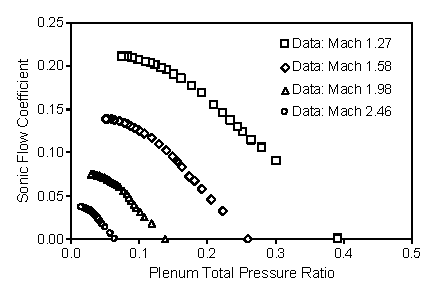
\includegraphics[width=3in]{willis_data_uncollapsed.eps}
     \caption{\LaTeX\ a very simple document from \cite{Slater2012}, who took it from \cite{Willis1995} Compile a very simple document.}
     \label{fig:MyFirstLaTeX}
 \end{center}
 %\vspace{-0.2 in}
\end{figure}

For each Mach number, the $Q_\trm{sonic}$, and so, the bleed flow $\mdot_\trm{bleed}$, increases as the plenum total pressure ratio is reduced. At some ratio, the bleed holes choke, and a maximum bleed rate is achieved. \cref{fig:MyFirstLaTeX} illustrates the decrease in $Q_\trm{sonic}$ as the Mach number increases. This reflects the increased losses and increased difficulty in bleeding the flow as the Mach number increases.

The bleed hole sonic mass flow coefficient, Qsonic is determined as function of the bleed hole angle, the bleed plenum pressure, and the local flow proprties. 

$$ Q_{sonic} = \frac{\dot{m}_{actual}}{\dot{m}_{max}} = f\qty(\alpha_{bleed},M_{local},\dfrac{P_{plenum}}{P_{Tlocal}}) $$

where $\dot{m}_{max}$ is the max theoretical flow at the local stagnation pressure and stagnation temperature. The local flow properties are taken at the wall for the inviscid flows or from the grid point that is just beyond the edge of the boundary layer for viscous flows. The q-sonic coefficient is a look-up table from the works of Syberg \cite{Syberg1973} and McLafferty \cite{McLafferty1958}.

Based on the definition for Qsonic and accounting for the surface pororisity $\Phi$, the effective bleed velocity magntitude is computed. The bleed flow is assumed to be normal to the flow domain boundary


% -----------------------------------------------------------
\section{Mayer and Paynter}

Mayer and Paynter \cite{Mayer1994} created a model treats each bleed region like a porous wall extending from the front edge of the bleed band to the afte edge. The flow velocity normal to the wall is computed based on the local flow properties, the total bleed hole area, and a discharge coefficient function. The model yields the overall effects of bleed mass removal on the inlet flow but does not completely model local variations in bleed that undoubtely exist in either the streamwise or cross-stream direction. The model is based on the assumption that removing the correct amount of mass from the inlet as the normal shock moves forward over the simulated prous bleed region is much more important in an accurate simulation of the motion of the normal shock than how the mass flux removal is distributed over a bleed region.

The surface porosity is calculated $\Phi$, the wall velocity is computed, and the bleed hole sonic mass flow coefficient $Q_{sonic}$ is determined as a function of the bleed hole angle, the bleed plenum pressure, and the local flow proprties. $Q_{sonic}$ is interpolated from Syberg \cite{Syberg1973} and McLaugherty \cite{McLafferty1958}. pulled from a lookup table and bilinear interpolation is used to calculate the appropriate values of Qsonic.

The bleed model of Mayer and Paynter17 stands out as representing the current state of porous bleed modeling. This model was implemented within the Wind-US CFD code.23 The inlet analyses of Ref. 13 illustrated the use of this bleed model for a supersonic inlet analysis. The model allows the bleed rate to vary across the bleed region according to local conditions. This is important when shock waves are interacting with the bleed region. For example, behind the shock wave, the static pressures are greater, which should result in a greater amount of bleed flow than ahead of the shock. The local bleed rate is calculated by extracting flow properties from the flow field and using a table look-up of empirically-based sonic flow coefficients, Qsonic. The use of the Qsonic data for the bleed model requires the CFD code to compute the Mach number, total pressure, and total temperature at the edge of the boundary layer. However, it may be computationally complex and time-consuming to locate each grid point at the boundary layer edge. This has can be especially difficult for unstructured-grid CFD codes. Further, the edge of the boundary layer may not be well-defined, such as in the case of a shock / boundary layer interaction with extensive boundary layer separation. Thus, a different approach for using the Qsonic data is needed.


%$$ u_{bleed} = \qty|u_{bleed}|n_{wall} $$

%Now the velocity on the boundary is set to the vector sum of the wall velocity and the bleed velocity

%$$ u = u_{wall} + u_{bleed} $$

%completing the application of the bleed boundary condition.

% -----------------------------------------------------------
Slater \cite{Slater2009} developed a model for 90 degree bleed holes based on the Willis data for single-hole data where there is interaction between adjacent holes.


% -----------------------------------------------------------
%\section{Slater Model}
% note
\section{FIBE Effort}

A renewed effort at NASA Glenn led to some experimental work. 

from eichorn paper

The similarity of the normalization curves for the different Mach numbers has led the authors to seek a scaling that would collapses the curves to a single distribution. Initial efforts by Davis4 and Slater1 focused on the $90^\circ$ data of Willis et al. Both investigators took the approach of normalizing the bleed plenum pressure by the local surface static pressure, but Davis also included a coefficient to account for the slight overpressure of the bleed plenum at zero flow rates. For scaling the flow coefficient, the investigators took different approaches. Whereas Slater assumed for the $90^\circ$ hole case that the total pressure in the hole was approximately equal to the local surface static pressure, Davis established a purely empirical scaling based on the extrapolated choked value of the bleed plate. Slater’s correlation takes the form of:

% -----------------------------------------------------------
\subsection{Slater Model}


$$ Q_{scaled} = \minus c \cdot \qty(P_{plen, scaled})^2 + b\cdot \qty(P_{plen, scaled}) + a$$


\begin{table}[!htbp] \centering 
\begin{tabular}[c]{*{2}{c}} \hline
\textbf{Coefficient} & \textbf{Value}   \\ \hline
a   & 0.59799735  \\ 
b   & 0.03069346  \\ 
c   & 0.59361420  \\ \hline
\end{tabular} 
\caption{Grid refinement in the plenum and patch sizing} 
\label{tab:slater} \end{table}

$$ P_{plen,scaled} = \dfrac{\qty(\dfrac{P_{plen}}{P_{t,e}})}{\qty(\dfrac{P_w}{P_{t,e}})} = \dfrac{\qty(\dfrac{P_{plen}}{P_{t,e}})}{\qty(1+\dfrac{\gamma-1}{2}\cdot M^2_e)^{\frac{\minus\gamma}{\gamma-1}}} $$

%$$ \dfrac{\qty(\dfrac{P_{plen}}{P_{t,e}})}{\qty(1+\dfrac{\gamma-1}{2}\cdot M^2_e)^{\dfrac{-\gamma}{\gamma-1}}} $$

$$ Q_{scaled} = \dfrac{Q}{\qty(\dfrac{P_w}{P_{t,e}})} = \dfrac{Q}{\qty(1+\dfrac{\gamma-1}{2}\cdot M^2_e)^{\frac{\minus\gamma}{\gamma-1}}} $$



The current work improves on the Mayer-Paynter bleed model by introducing a scaling of the Qsonic data for 90-degree bleed holes. The scaling is able to collapse the Qsonic data for various Mach numbers to a trend that can then be fitted with a quadratic polynomial which is only a function of the ratio of plenum static pressure to the surface static pressure. The scaling eliminates the requirement to compute the flow properties at the edge of the boundary layer. The curve fit also provides a rudimentary model for blowing within a bleed region, which can occur if there is recirculation within the bleed region in the presence of a shock. The next section discusses the bleed modeling and the scaling of the Qsonic data. The improved bleed model was implemented into the Wind-US CFD code

The porous bleed boundary condition is imposed for surface grid points located within the bleed region. The model assumes the region is continuously porous, and so, the flow through individual holes is not resolved nor are individual holes recognized.

The ability of the bleed holes to extract bleed flow is represented by the sonic flow coefficient Qsonic. The bleed flow rate is calculated in the form of

The W is the flow rate given in the general form of $ W = \rho A v $

The Wsonic is calculated by assuming isentropic conditions through the bleed holes with sonic flow (M = 1) within the bleed holes.

in summary, 


A quadratic curve was fitted to the scaled data of Fig. 2. The quadratic equation is

Figure 2 indicates that at a static pressure ratio of approximately 1.03, the bleed flow is zero. The plenum pressure is slightly higher than the surface static pressure. The fact may indicate a dynamic or ram effect of the flow into the bleed holes, even at 90 degrees. As the static pressure ratio approaches zero, the surface sonic flow coefficient approaches 0.6. This reflects the loss incurred in turning the flow into the bleed hole. Figure 3 shows the application of the scaling to sonic flow coefficient data sets used in references 2 and 17. There is greater variation in the scaled values than shown in Fig. 2, but the curve fit of Eq. 13 does well in characterizing the data. The exception is the data for Mach 1.0 where the curve fit indicates lower values for the surface sonic flow coefficient. Note that the minimum Mach number of Fig. 1 upon which the curve fit was generated was Mach 1.27. The comparisons of Fig. 3 suggest that the curve fit may not work well for characterizing bleed rates below Mach 1.27. This is under continued study; however, given that most of the flow in supersonic inlets is above Mach 1.27, the curve fit should provide a good characterization of the bleed flow in supersonic inlets.

An additional benefit of the scaling of the sonic flow coefficient as expressed in Eq. 13 is that it provides a rudimentary model for blowing in a bleed hole. When the static pressure ratio is greater than 1.03, the value of the surface sonic flow coefficient is negative, which by Eq. 2 will result in a negative bleed flow or blowing. While large amounts of blowing are not intended in the design of a supersonic inlet, it is possible to experience recirculation within a bleed region. This can occur when a shock wave is interacting with the bleed region and the total bleed flow for the bleed region is small. The high pressures downstream of the shock cause pressurization of the bleed plenum, which forces the bleed plenum to blow flow out the bleed holes upstream of the shock where the local pressures are lower.



% -----------------------------------------------------------
\subsection{Slater Model Modified}
% from slater journal paper

The original slater model yields a positive slope as $p_{plenum}/p_B < 0.02585 $, contradicting the expectation that the sonic flow coefficient continually increases as the static plenum pressure approaches zero.

by Andrew Dorgan of the Boeing Company, private communications, Apr. 2011

$$ Q_{sonic-B} = -0.57 \cdot \qty(\frac{p_{plenum}}{p_B})^2 $$

This alternative curve-fit differs in shape only slightly and not distinguishable if plotted.

%These models provide a rudimentary model for blowing in a bleed hole.

% -----------------------------------------------------------
\subsection{Davis Model}

and Davis' scaled empirical correlation takes the form of:

% from eichorn paper

$$ Q_{scaled} = a + \dfrac{b}{1+\qty(\dfrac{P_{plen,scaled}}{c})^d} $$

\begin{table}[!htbp] \centering 
\begin{tabular}[c]{*{2}{|c}|} \hline
\textbf{Coefficient} & \textbf{Value}   \\ \hline
a   & -0.74177271 \\ \hline
b   &  1.7397157  \\ \hline
c   &  0.91473254 \\ \hline
d   &  3.2074431  \\ \hline
\end{tabular} 
\caption{Grid refinement in the plenum and patch sizing} 
\label{tab:davis1} \end{table}

where 

$$ P_{plen,scaled} - \frac{\dfrac{P_{plen}}{P_{t,e}}}{1.059\cdot\dfrac{P_w}{P_{t,e}}} = \dfrac{\qty(\dfrac{P_{plen}}{P_{t,e}})}{1.059 \cdot \qty(1+\dfrac{\gamma-1}{2}\cdot M^2_e)^{\sfrac{\minus\gamma}{\gamma-1}}} $$

$$ Q_{scaled} = \dfrac{Q}{e + f\cdot M_e^2 + g \cdot e^{M_e}} $$

\begin{table}[!htbp] \centering 
\begin{tabular}[c]{*{2}{|c}|} \hline
\textbf{Coefficient} & \textbf{Value}   \\ \hline
e   & -6.885241  \\ \hline
f   & -5.9569877 \\ \hline
g   &  5.9532869 \\ \hline
\end{tabular} 
\caption{Grid refinement in the plenum and patch sizing} 
\label{tab:davis2} \end{table}

Davis \cite{Davis2012} concluded that the scaling method presented by Slater (Ref. 4) was a better, but imperfect, fit for single-hole data than the scaling method Davis has previously proposed based upon a semi-empirical correlation of the data collected by Willis.

% -----------------------------------------------------------
\subsection{Results from Phase I}
% note
strenghts and weaknesses of slater model. can include plot from eichorn paper

Both methods collapse the $90^\circ$ data fairly well. The plot shows Elater's correlation fits the present data better which isn't unexpected since Davis' correlation was based on an empirical fit of the extrapolated choke points of the multi-hole data. Slater's correlation seems to fit the lower Mach number data better with increasing deviation as the Mach number is increased. However, even the lowest Mach number data deviation from the Slater correlation near the choke point, implying that n adjustment for the number of bleed hole rows, and potentially the hole spacing, may be required.

The above wall static pressure scaling (slater) assumes that the total pressure in the hole is nearly the same as the surface wall static pressure. This is likely a reasonable assumption for holes with large inclination angles as all the freestream total pressure is lost turning the flow through a large angle. As the inclination angle is reduced, however, some of the freestream total pressure is expected to be recovered in the hole and it is thus expected that the above scaling will not work as well, particularly at high flow rates. This suggests that a physics-based model must account for the total pressure recovery in the hole which may be a function of a number of parameters.

% -----------------------------------------------------------
\subsection{Results from Phase II}
Davis \cite{Davis2012} and Eichorn \cite{Eichorn2013} present Phases I and II, respectively, of a Fundamental Inlet Bleed Experiments study at NASA Glenn Research Center.

Several examples of collapsed data using the equations above for specific bleed holes are given in Figure 7. Unlike the data collected by Davis (Ref. 6), the data from many of these plates collapse very well when this scaling is applied. Of particular note are plates with the smallest nominal thickness-todiameter ratio (t/D=0.25), Figure 7(a) to (c) (top row of plots), which collapse very well independent of hole angle. That these plates collapse well isn’t necessarily surprising inasmuch as very thin plates do not have the same internal shock structure as thicker plates do. Figure 7(d) to (f) (middle row of plots) display the collapse for hole configurations where the nominal thickness-to-diameter ratio is 2.0 and the hole angle is $55^\circ$ and in this case the collapse appears to have higher degree of scatter, however there is little apparent trend in Mach number. The final selection, Figure 7(g) to (i), present the $20^\circ$ hole data and as Davis (Ref. 6) concluded, the scaling does not work particularly well for $20^\circ$ holes. These have a distinct difference in magnitude where the maximum scaled sonic flow coefficient increases with Mach number. Further this tendency is related to the hole diameter as the smaller hole diameters show less separation between the curves.

A comparison of all collapsed data is shown in Figure 8. The values for the $20^\circ$ holes are noticeably larger than those of the $90^\circ$ and $55^\circ$ holes which themselves form two distinct groups. The $90^\circ$ holes seem to form tight bands for specific thickness-to-diameter ratios, however both the $55^\circ$ and $90^\circ$ holes only show a loose grouping where that ratio is small.


% notes
from slater conf paper

The methods of computational fluid dynamics (CFD) have been applied to the aerodynamic analysis of supersonic inlet flows containing bleed regions.11-13 The small scale of the bleed holes has resulted in the typical approach of modeling the effects of porous bleed through the use of surface boundary conditions. Various bleed boundary condition models have been reported by a number of researchers.14-22 These models follow the general approach of assuming the bleed region to be a continuously porous surface. The solution points located within the bleed region are computed as boundary conditions in which the local bleed rates and velocity components are computed. The individual bleed holes are not identified nor are the details of the flow within the bleed holes computed. The models attempt to capture the collective behavior of the bleed holes.



% -----------------------------------------------------------
\section{Experiment}
% from Slater conf paper


The experiment \verb|cite willis davis hingst| that was used for validation was performed in the NASA Glenn Research Center 1 ft by 1 ft Supersonic Wind Tunnel (SWT) measuring mass flow rate through bleed holes at various Mach numbers. The quantities that were used in the validation were the boundary layer thickness and momentum thickness of the naturally boundary layer along the wind tunnel wall, the bleed hole diameter, the bleed hole depth, and the pressure ratios used in the experiment to draw air through the bleed hole. A plenum sat below the hole where the plenum pressure could be varied (which controlled the pressure ratio through the hole), varying the massflow rate through the hole.

D = 0.236 in.
L = 2D

\begin{table}[!htbp] \centering 
\begin{tabular}[c]{*{2}{l}} \hline
\textbf{Parameter} & \textbf{Value}   \\ \hline
Mach Number   & 2.46  \\ 
Total Pressure [psia]   & 25.0 \\ 
Reynolds Number per foot   &  5.15E+06 \\ 
Boundary Layer Thickness [in.] & 0.5079 \\ \hline
\end{tabular} 
\caption{Grid refinement in the plenum and patch sizing} 
\label{tab:bl} \end{table}

\begin{table}[!htbp] \centering 
\begin{tabular}[c]{*{5}{c}} \hline
\textbf{Parameter} & \textbf{Value} & \textbf{Grid Size} & \boldmath{$Q_{sonic}$} & \boldmath{$\Delta Q_{sonic}$}    \\ \hline
SA & 0.08 & Small & 0.0273 & 5.52\% \\ \hline
\end{tabular} 
\caption{Grid refinement in the plenum and patch sizing} 
\label{tab:grid_convergence} \end{table}

the hole was located in a disc mounted flush with the bottom of the test section of the 15- by 15-cm wind tunnel at the NASA Glenn Research Center. The boundary layer over the plate was the naturally occuring Boundary layer on the bottom surface of the tunnel.

The CFD simulations involved a single 90-degree bleed hole with a diameter D = 0.236 inches and length of L = 2 D. The hole was located in a disk mounted flush with the bottom of the test section of the 15cm x 15cm wind tunnel at the NASA Glenn Research Center. The boundary layer over the plate was the naturally-occurring boundary layer on the bottom surface of the wind tunnel. The flow conditions and boundary layer profile approaching the bleed region were measured with a translating pitot probe and wall static pressure ports. The reference station for the approach flow was located 2.46 inches ahead of the center of the bleed hole. The bleed plenum was attached to the outside of the wind tunnel with ducting to a vacuum exhaust. The plenum was cylindrical with an inside diameter of 2.874 inches and an axial length of 3.50 inches. The axis of the plenum was parallel to the axis of the bleed hole. A vacuum chamber was used to establish the bleed flow rate, which was measured using a calibrated nozzle. The uncertainty of the experimental data was reported as $\pm1.5 \%$ for total pressures, and $\pm 1 \%$ percent for values of Qsonic. 

The CFD simulations were performed at a Mach number of 2.46. The side-view and front-view of the computational flow domain are shown in Fig. 6. The bleed hole and plenum are located below the tunnel and shown at the bottom of Fig. 6. Geometric and flow symmetry was assumed and allowed only half of the tunnel, bleed hole, and plenum to be simulated. A reflection boundary condition was used on the symmetry plane. The bottom and side of the tunnel were specified with adiabatic, no-slip boundary conditions. The top of the tunnel was specified as an inviscid wall so as to require less grid points to resolve the boundary layer, which was assumed not to influence the flow through the bleed hole. The inflow boundary was positioned an axial distance of 38.46 inches ahead of the center axis of the hole. This position was determined to provide a turbulent boundary layer at the reference location that matched the reference boundary layer profile and edge conditions of the experiment. The  conditions at the edge of the boundary layer were a Mach number of 2.46, total pressure of 25.0 psia, and a Reynolds number of 5.15E+06 / ft. The boundary layer thickness was 0.5079 inches. The outflow boundary was positioned 5.0 inches downstream of the center axis of the bleed hole and a first-order extrapolation boundary condition was used for the supersonic outflow. The plenum was modeled as a cylinder with a converging-diverging nozzle directed downward for the outflow for the plenum. The exit for the plenum nozzle was located 6.472 inches below the bottom wall of the tunnel and a subsonic outflow boundary condition was imposed in which the static pressure was specified. The bleed flow reached very low speeds within the plenum and the intent of the nozzle was to create a smooth exit for the bleed flow from the plenum. The walls of the plenum and bleed hole were specified as adiabatic, no-slip boundary conditions.

Initial solutions for the tunnel boundary layer indicated that a wall spacing of 2.4E-04 inches provided a non-dimensional wall spacing of y+  1.0. The grid distribution was determined using a hyperbolic-tangent method with end-spacings specified. The number of grid points along an edge was selected such that the maximum grid stretching was less than $15\%$. Within the bleed hole, the maximum spacing was limited to 0.005 inches (0.02 D), which set the level of maximum resolution of the flow within the bleed hole. This grid established the highest resolution of the flow field for the grid convergence study (fine grid). The resulting grid contained 678375 grid points within the bleed hole. The entire grid contained over 6.66 million grid points with over half of the grid points located within 3 diameters of the bleed hole and within the plenum. 

The CFD flow solution was initialized with Mach 2.46 flow within the tunnel and very low speed (Mach 0.01) flow within the bleed hole and plenum with a static pressure equal to the tunnel static pressure. An inviscid boundary condition was imposed at the plenum nozzle exit so as to initially not allow any bleed flow. This created the zero-bleed solution. Flows with bleed were then simulated by imposing the subsonic outflow boundary condition at the plenum nozzle outflow and specifying reduced values of static pressure to draw out the plenum flow. Subsequently lower values of exit static pressure yielded a sequence of solutions with greater bleed flow until the maximum bleed flow was obtained with essentially a vacuum within the plenum. 

At each solution point, the iterative convergence was examined by monitoring the amount of bleed flow and the plenum static pressure. The bleed flow was measured within the plenum nozzle where the flow was entirely directed toward the exit without recirculation, which ensured an accurate evaluation of the mass flow. The plenum pressure was obtained by mass-averaging the static pressure on a horizontal plane near the start of the nozzle. 

The grid convergence was examined by solving the flow field on three grids of subsequent coarseness. The Wind-US code allows grid sequencing in which allows the solution to be computed on coarser grids obtained by skipping a number of grid points. This allowed the grid sensitivity study to be conducted without having to generate coarser grids. The medium grid was obtained by skipping every other grid point. The coarse grid was obtained by skipping three grid points. This can also be used to accelerate convergence by starting the initial solution on the coarse grid. Table 2 lists the results on the coarse (0.08D), medium (0.04D), and fine (0.02D) grids for both the Spalart-Allmaras (S-A) and Menter SST turbulence models. The simulations were performed with the bleed rate approximately $75\%$ of its maximum value. As can be seen, the bleed rates showed little variation between the medium and fine grids. This can also be seen in Fig. 8 with the plot of the data of Table 2. The value of Qsonic from the experiment is also plotted in Fig. 8. 

The simulations with the S-A and SST turbulence models are essentially the same with both indicating Qsonic values approximately $25\%$ higher than the experimental data. However, it was discovered that the approach Mach number for these simulations was only 2.38 rather than 2.46. The inflow conditions were subsequently changed to obtain the correct inflow Mach number of 2.46 for the remaining simulations. However, this did not change the conclusion that further simulations could be conducted using the medium grid with a resolution of 0.04 D using the Menter SST turbulence model. Figure 8 shows the result of simulation D which was conducted on the medium grid with the Menter SST turbulence model.

The flow conditions 

talk qualitatively about the physics in the hole

some issues that i faced was that the flow was very unsteady, probably due to a timestep issue. talk a lot about this

\begin{table}[!htbp] \centering 
\begin{tabular}[c]{*{5}{c}} \hline
& \textbf{Small Patch} & \textbf{Medium Patch} & \textbf{Large Patch} & \textbf{Complete Suction} \\ \hline
\textbf{Coarse Grid} & 14.8\% & 3.4\% & 11.1\% & 2.0\% \\
\textbf{Medium Grid} & 12.3\% & 4.6\% &  3.0\% & 1.8\% \\
\textbf{Fine Grid}   &  9.7\% & 2.2\% &  0.0\% & 1.5\% \\ \hline
\end{tabular} 
\caption{Grid refinement in the plenum and patch sizing} 
\label{tab:results} \end{table}


%\figSmallPatch

% ======================================================= Grid Independence
%\subsection{Grid Independence}

%\begin{figure}[tbp!] \centering
%	\begin{subfigure}{0.5\textwidth}
%		\centering
%		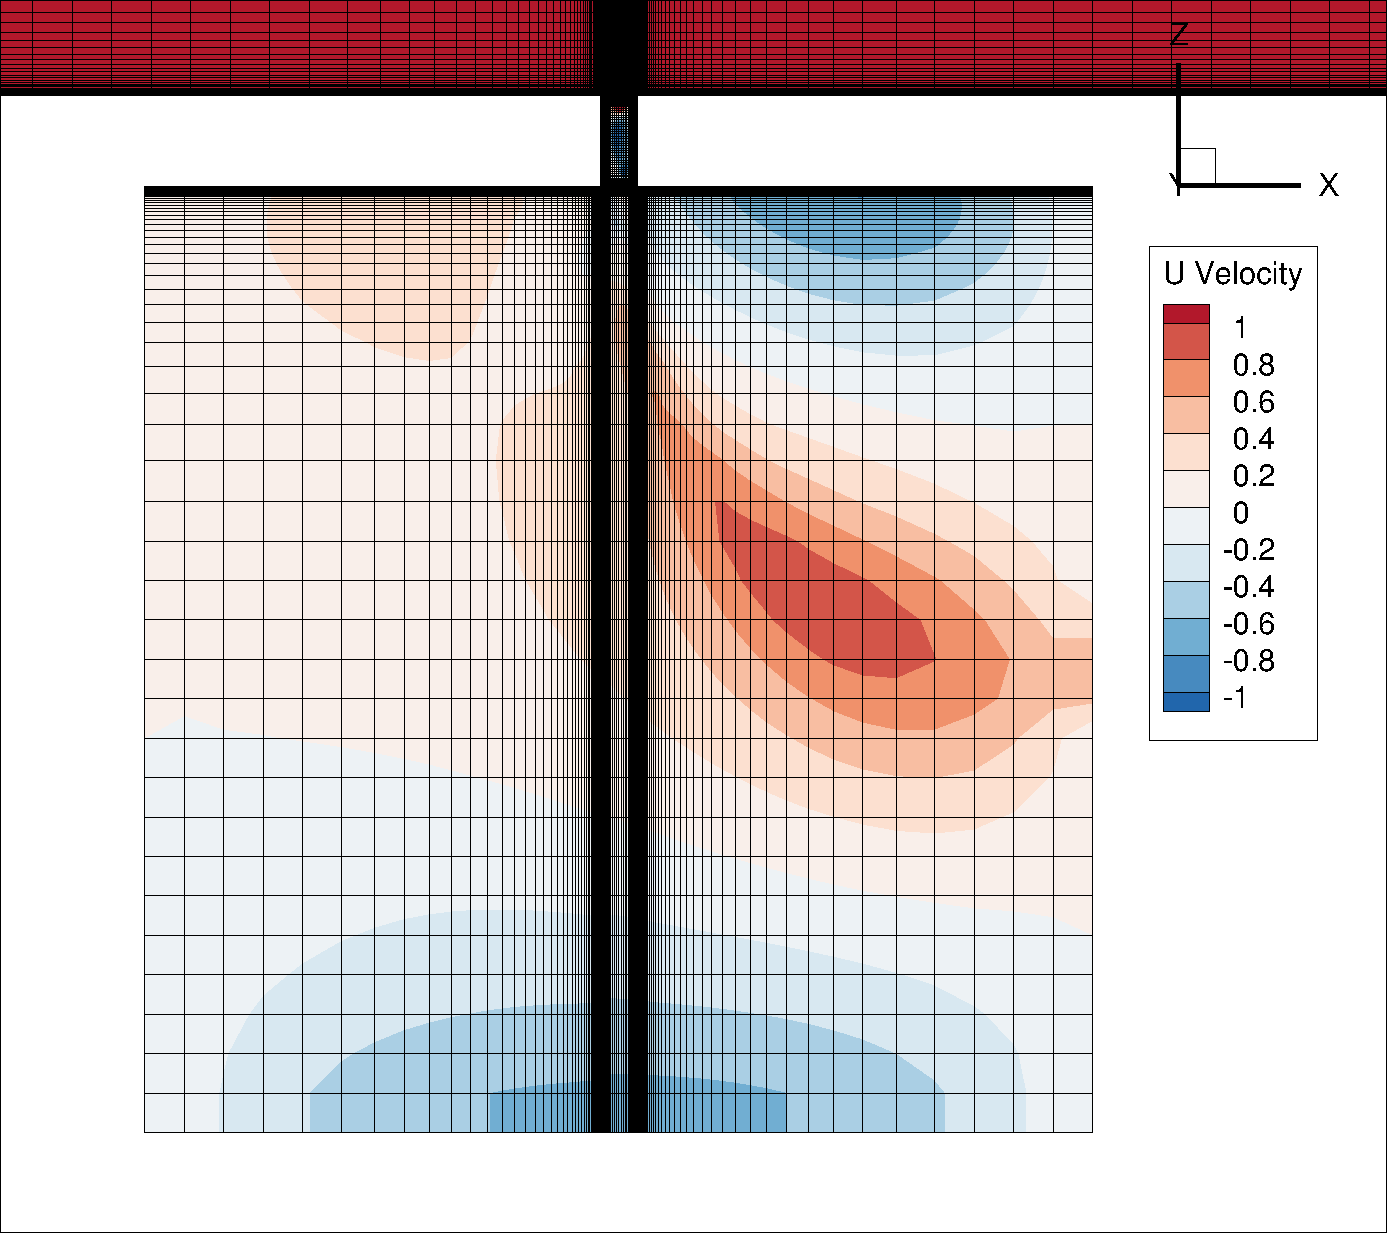
\includegraphics[width=0.5\linewidth]{1-1_grid.png}
%		\caption{1} \end{subfigure}%
%	\begin{subfigure}{0.5\textwidth} 
%		\centering
%		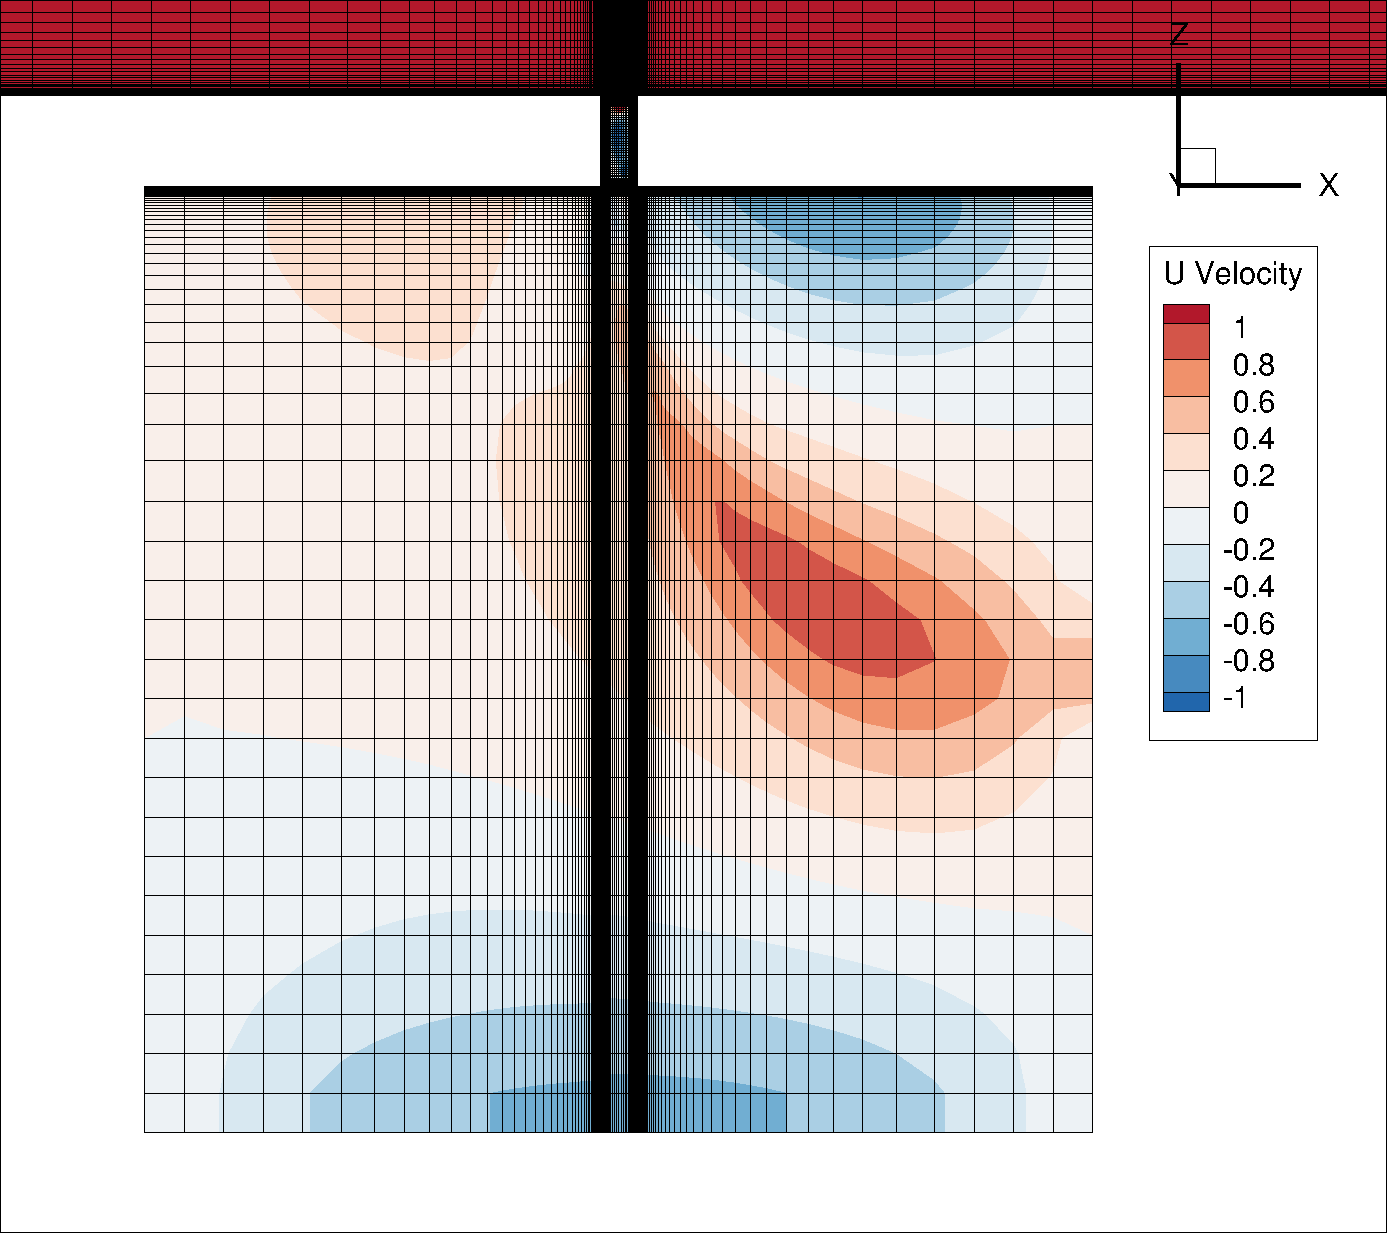
\includegraphics[width=0.5\linewidth]{1-1_grid.png}
%		\caption{1} \end{subfigure}
%\caption{hihi}
%\label{fig:small}
%\end{figure}

% \begin{figure}[tbp] \centering
% \begin{subfigure}{.32\textwidth} \centering
%   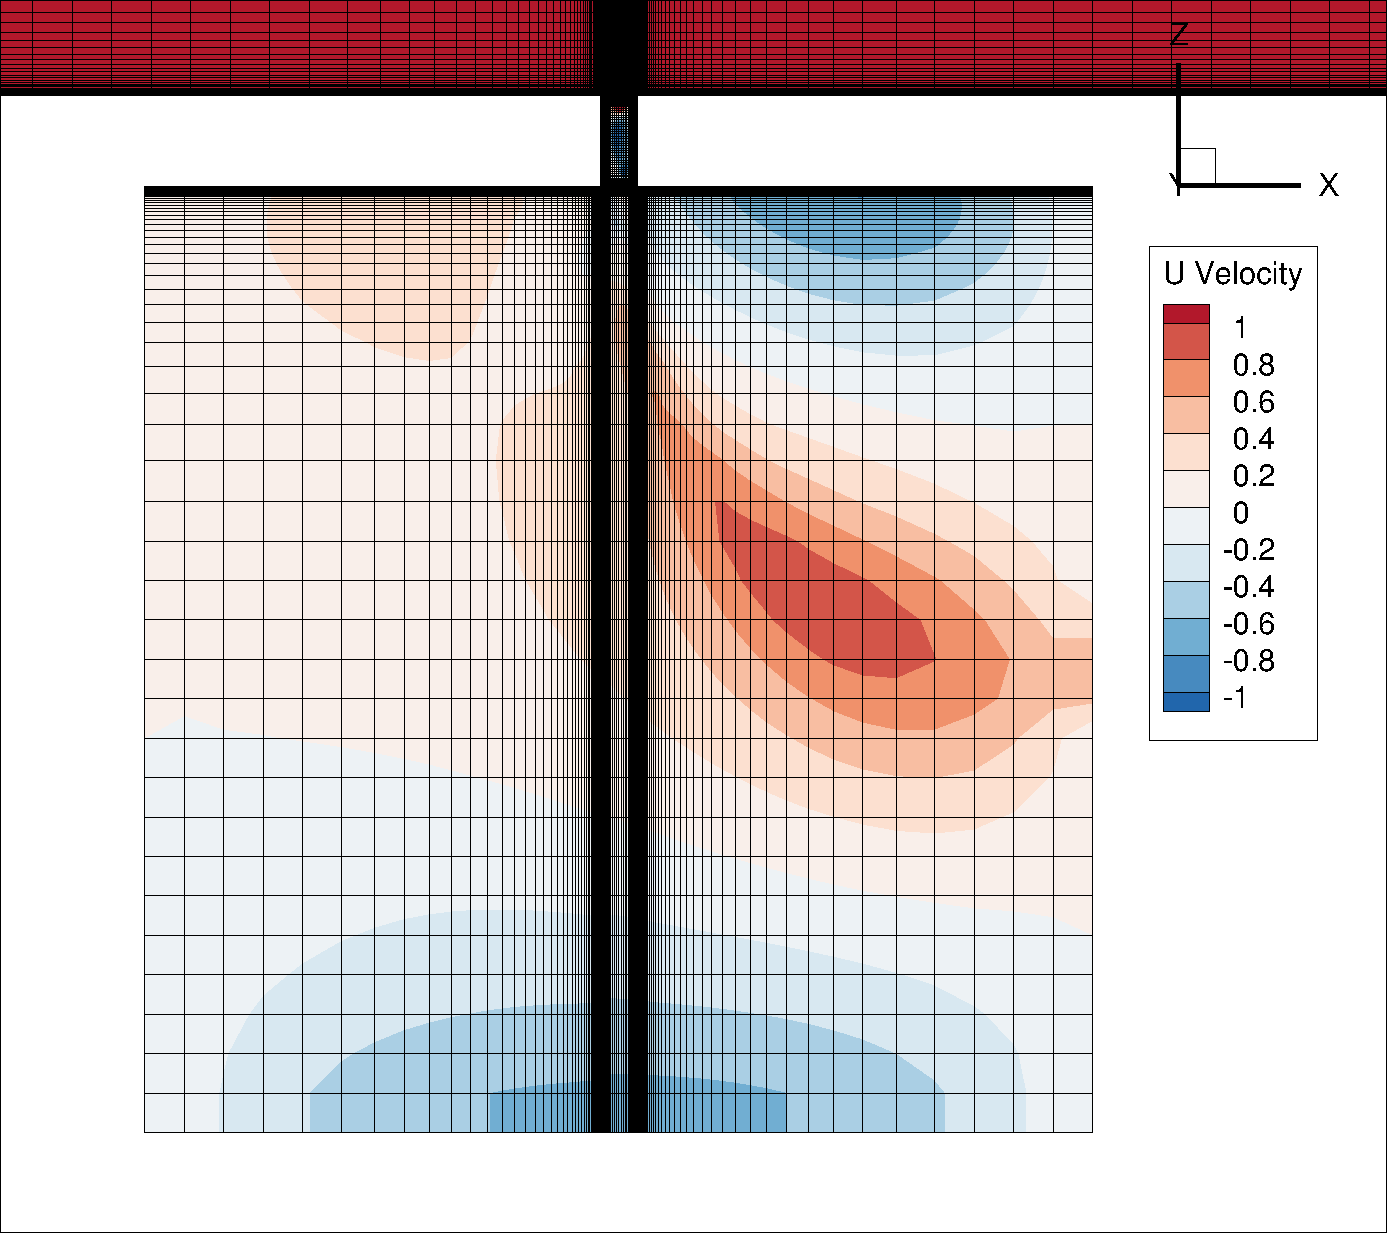
\includegraphics[width=1\linewidth]{1-1_grid.png}
% \end{subfigure}%
% \begin{subfigure}{.32\textwidth} \centering
%   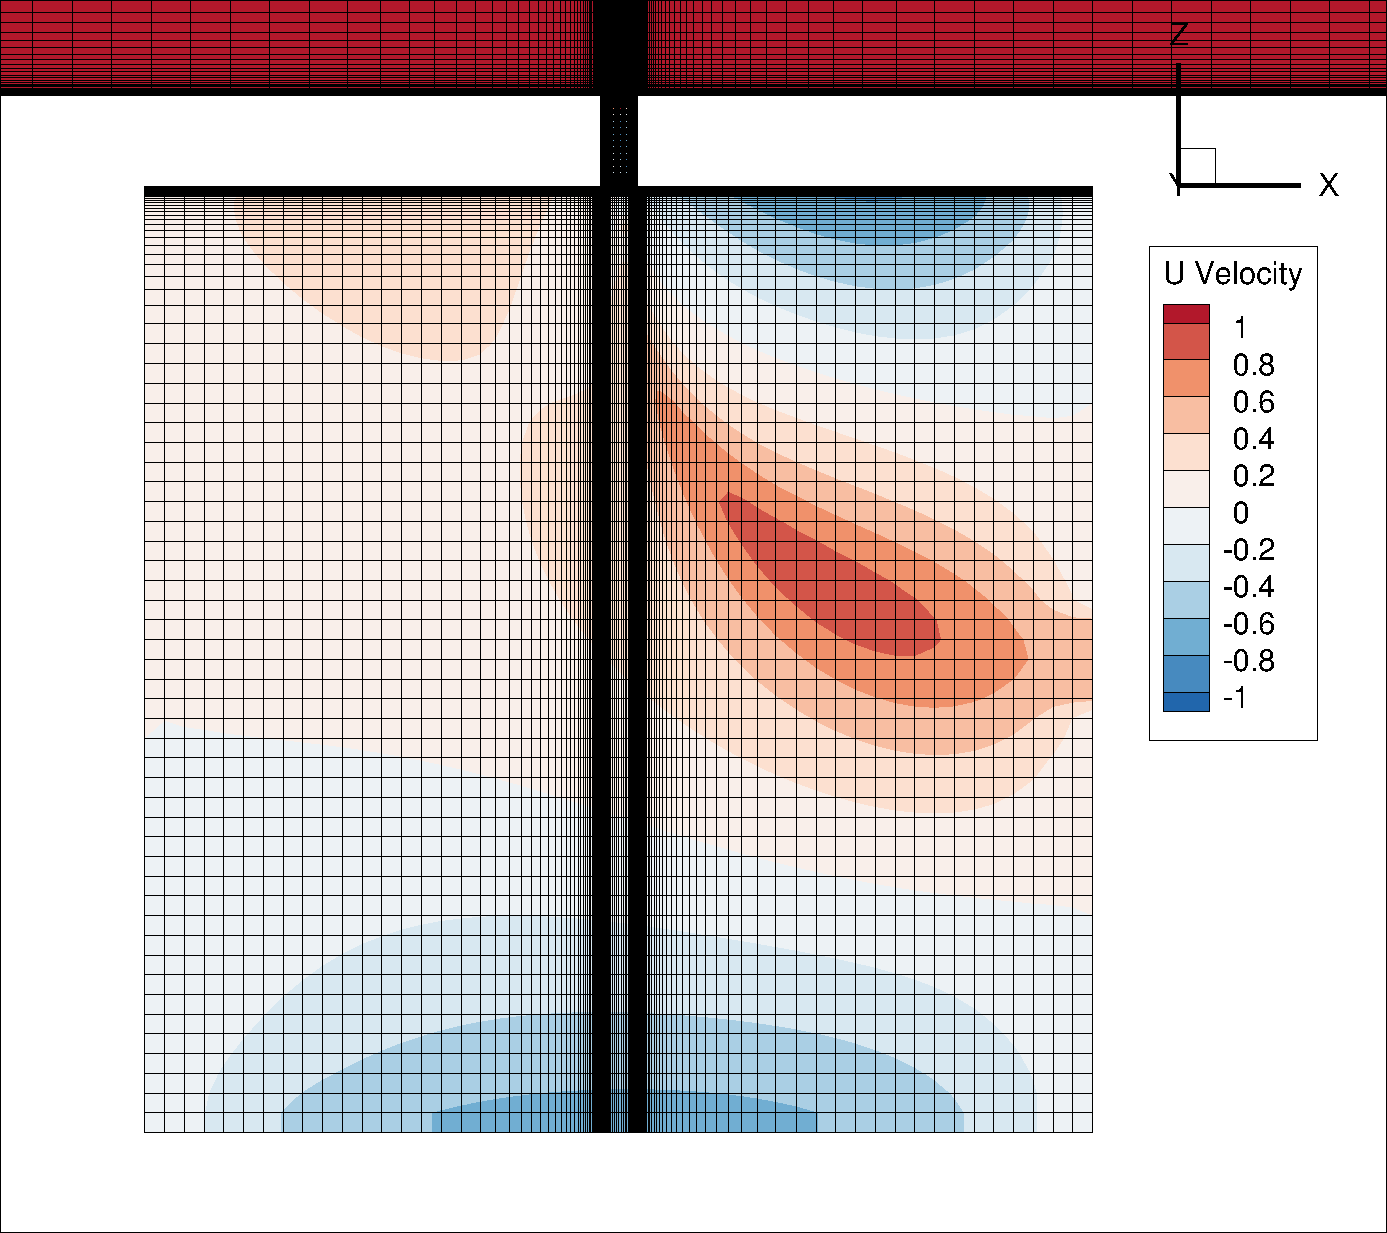
\includegraphics[width=1\linewidth]{1-2_grid.png}
% \end{subfigure}%
% \begin{subfigure}{.32\textwidth} \centering
%   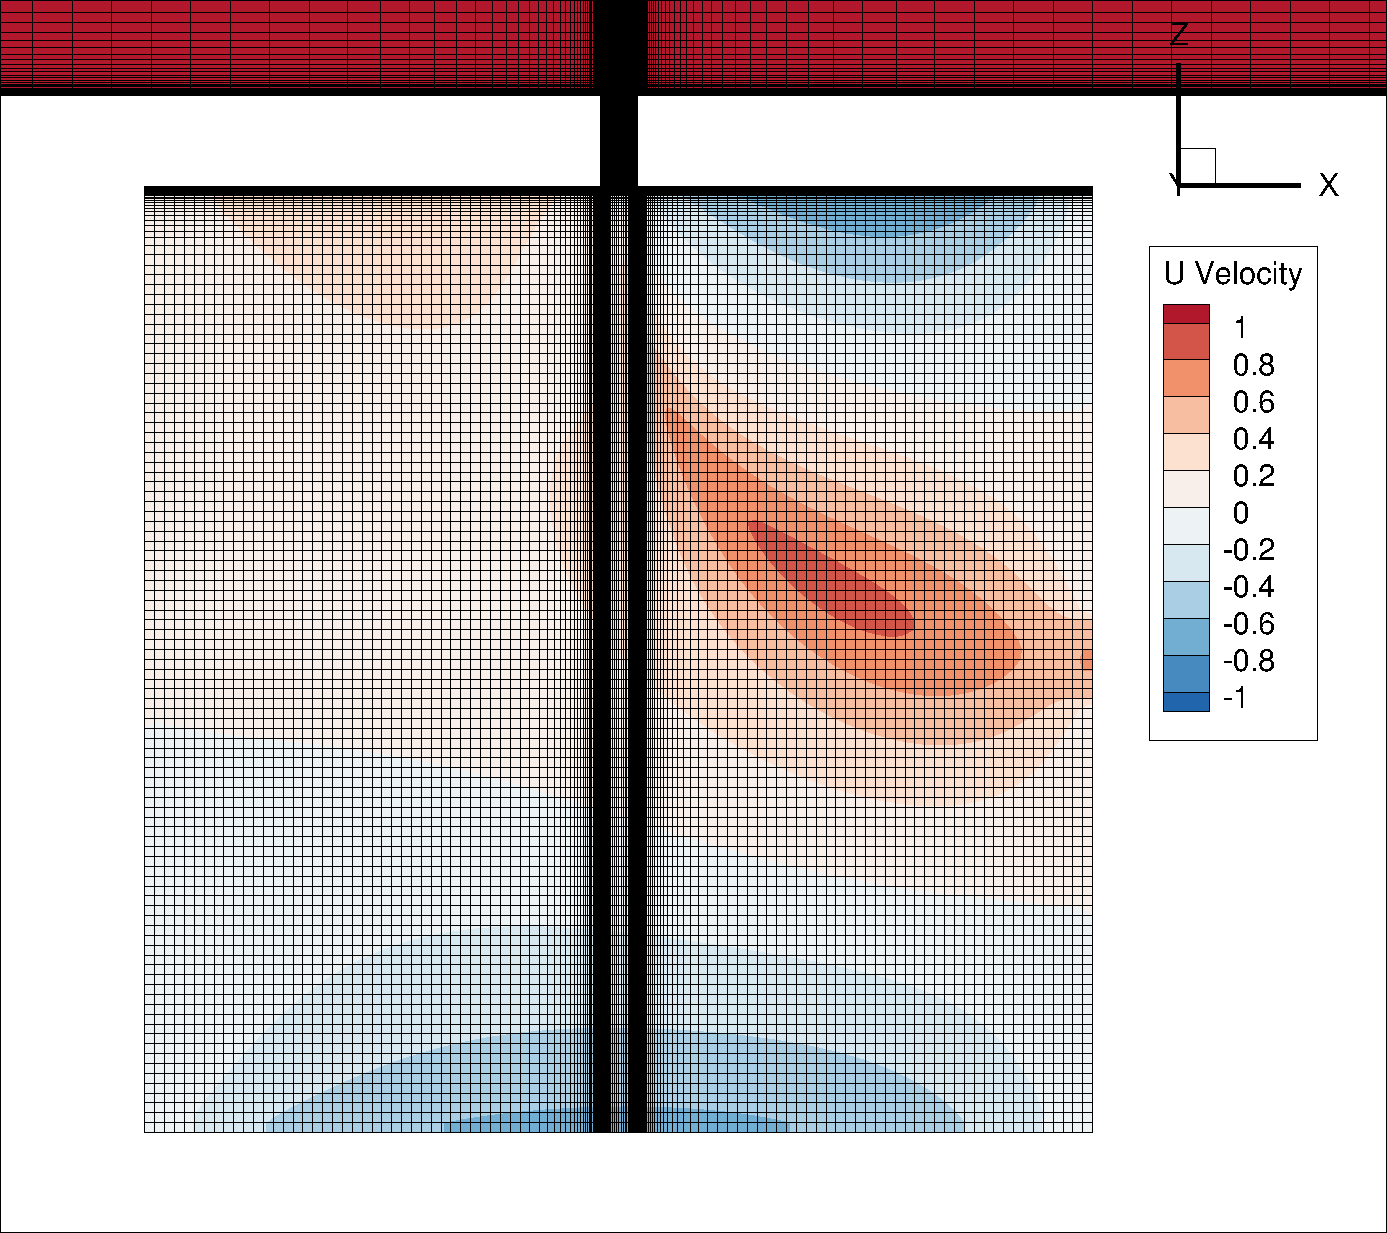
\includegraphics[width=1\linewidth]{1-3_grid.png}
% \end{subfigure}
% \begin{subfigure}{.32\textwidth} \centering
%   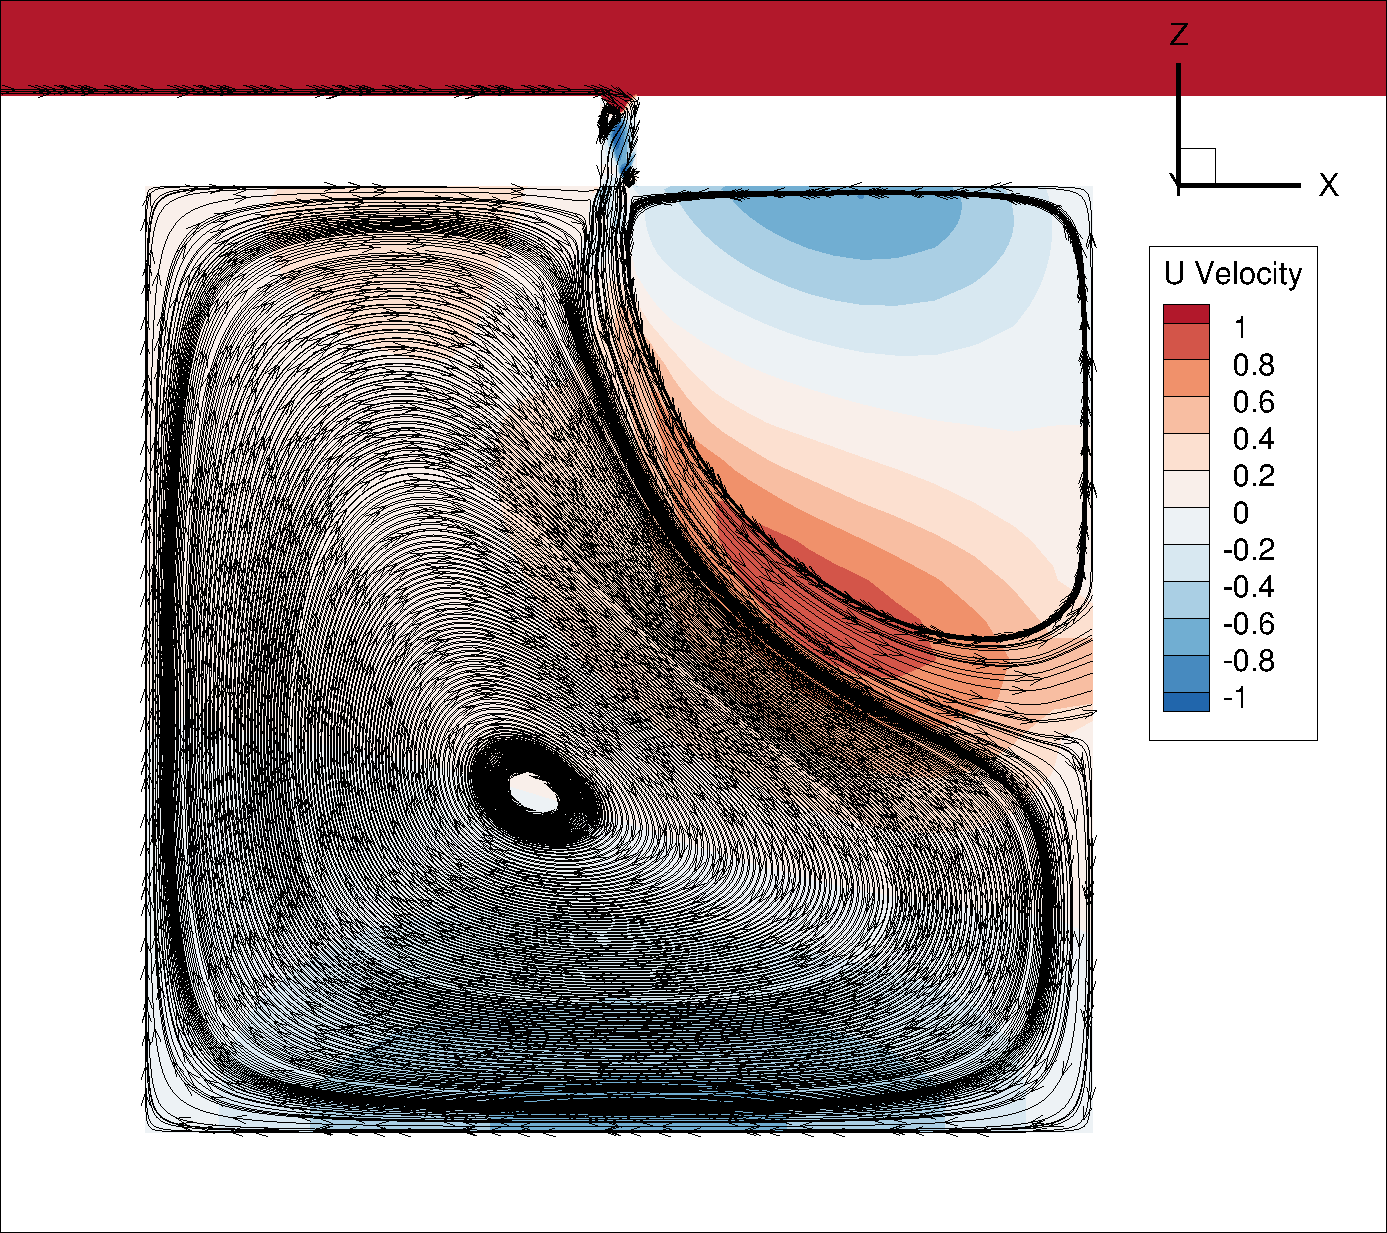
\includegraphics[width=1\linewidth]{1-1_streamlines.png}
% \end{subfigure}%
% \begin{subfigure}{.32\textwidth} \centering
%   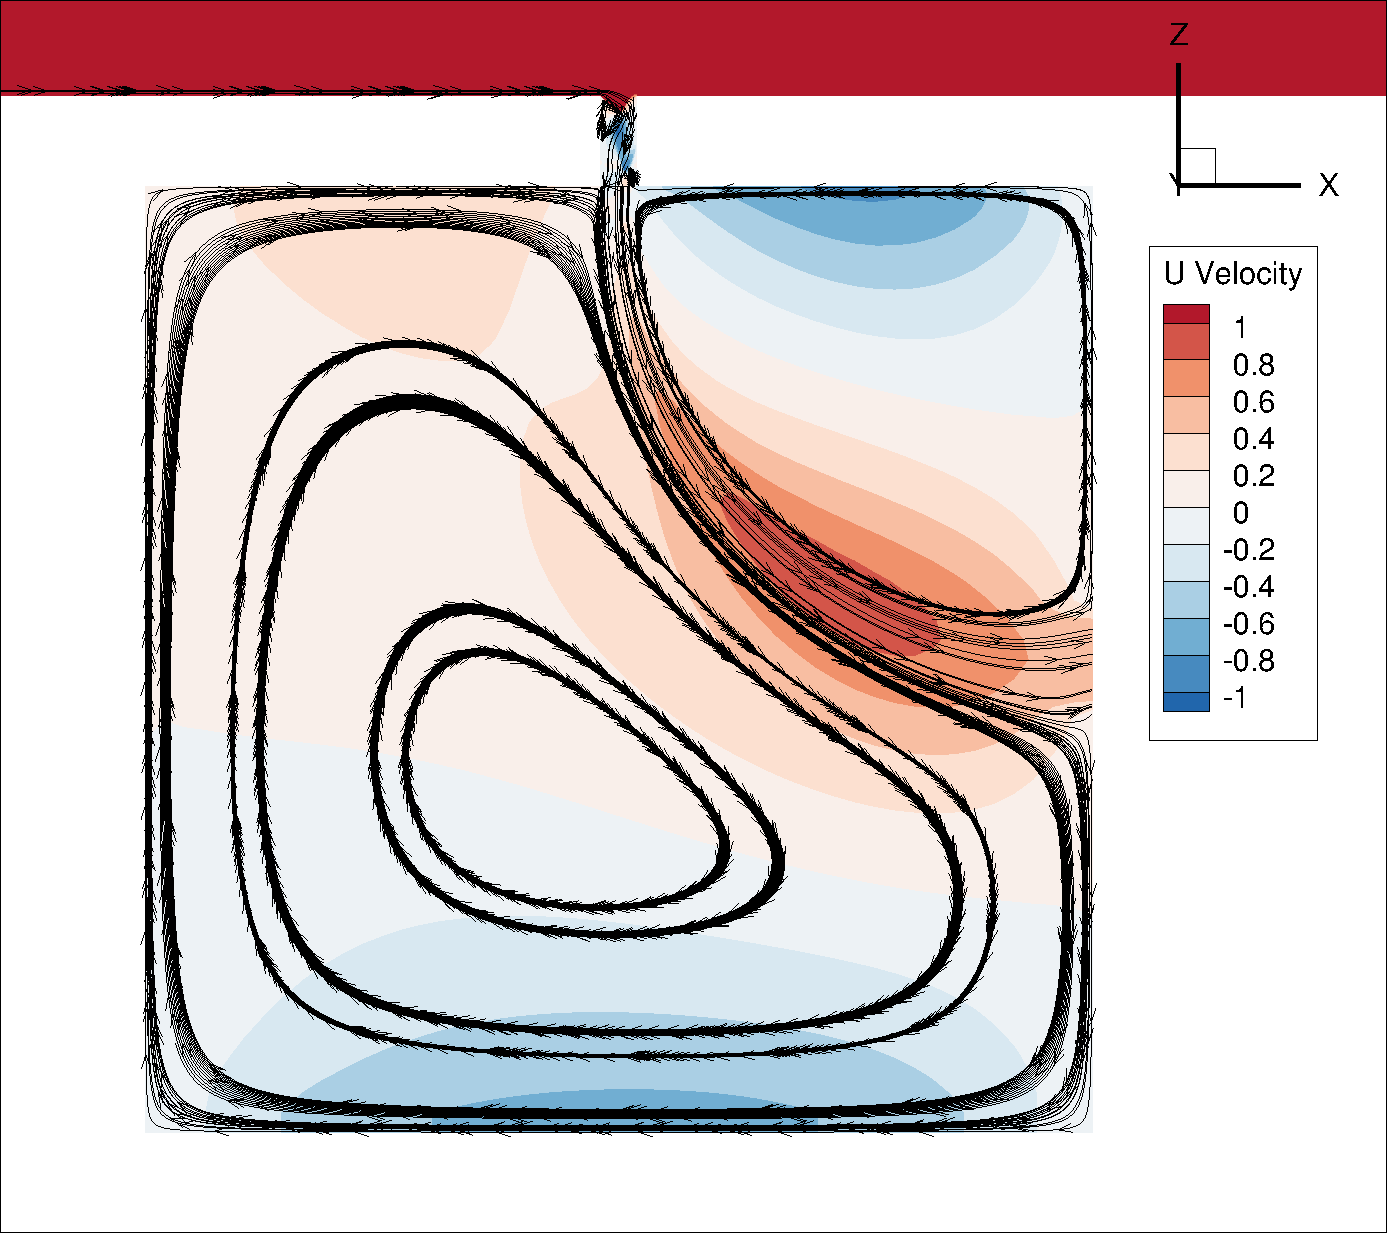
\includegraphics[width=1\linewidth]{1-2_streamlines.png}
% \end{subfigure}%
% \begin{subfigure}{.32\textwidth} \centering
%   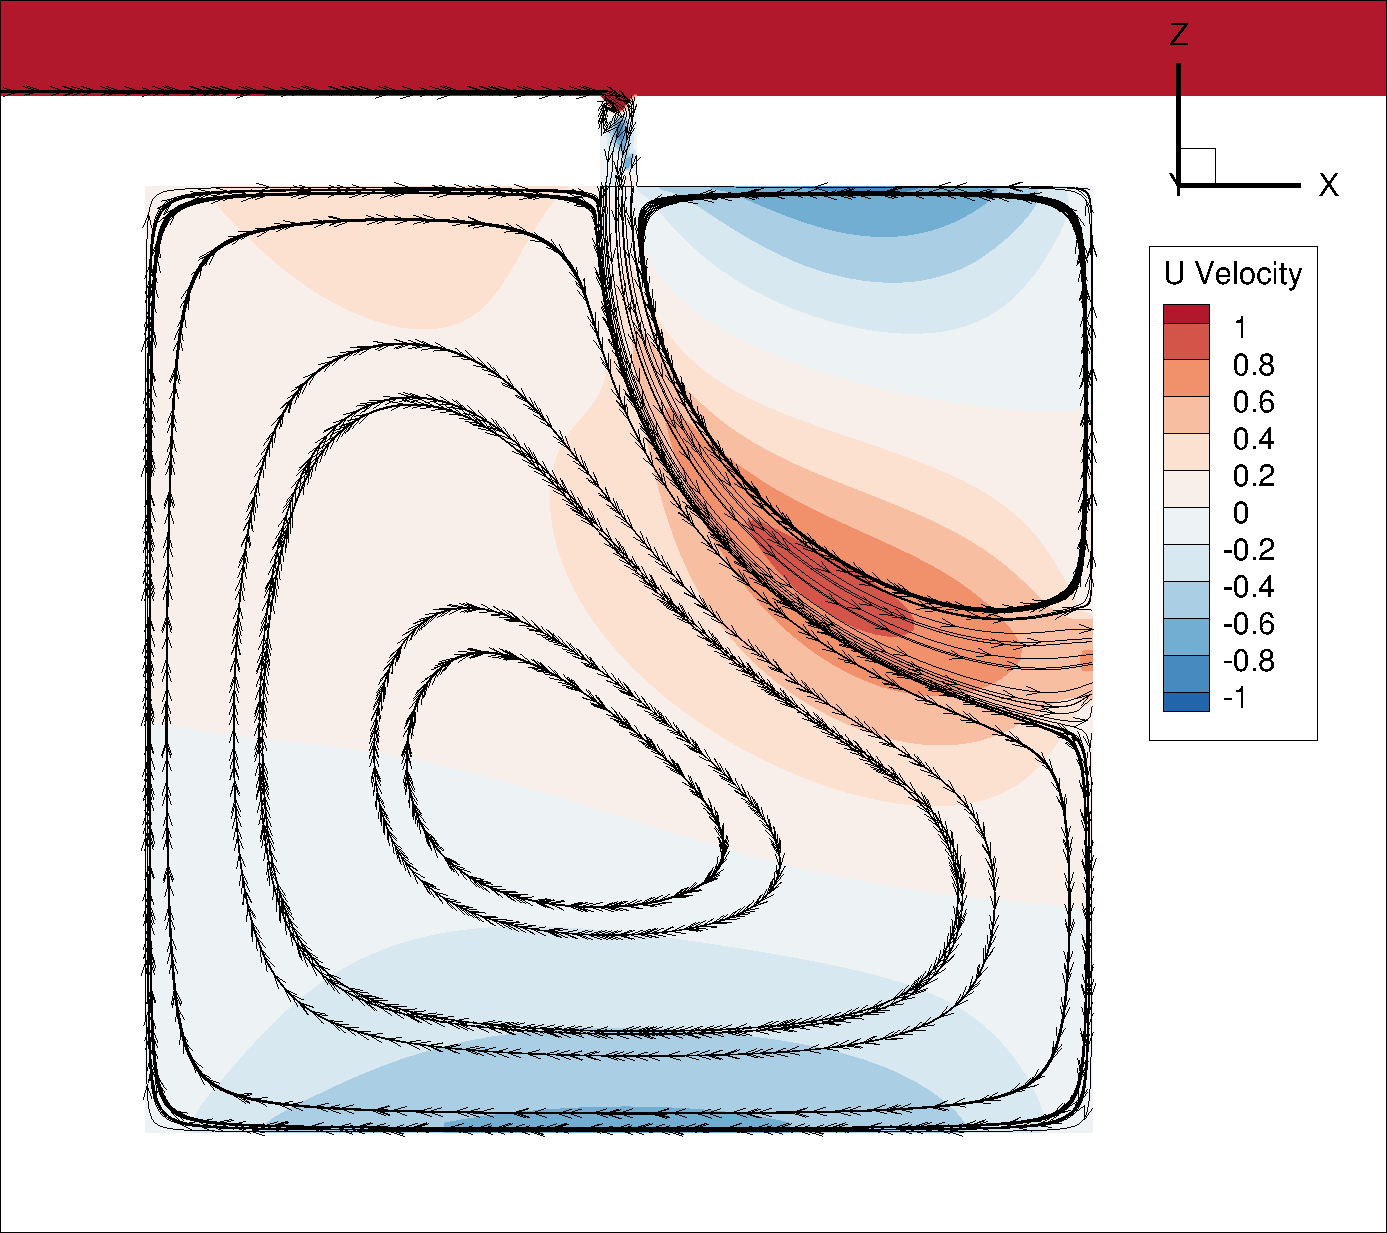
\includegraphics[width=1\linewidth]{1-3_streamlines.png}
% \end{subfigure}
%   \caption{Grid resolution study of the contours of u-velocity and streamlines for % the small patch}
%   \label{fig:small}
% \end{figure}

% ======================================================= Time Independence
%\subsection{Time Independence}

% ======================================================= Results
%\subsection{Results}
	%\section{Shock Unsteadiness Characterization}

% ======================================================= Grid Independence
\subsection{Grid Independence}

% ======================================================= Time Independence
\subsection{Time Independence}

% ======================================================= Results
\subsection{Results}
	%\section{Shock Mitigation Study}

% ======================================================= Grid Independence
\subsection{Grid Independence}

% ======================================================= Time Independence
\subsection{Time Independence}

% ======================================================= Results
\subsection{Results}

% ====================================================== Conclusion
	%\chapter{Conclusion} \label{conclusion}
	%% Chapter 05: Findings and Conclusions

\section{Findings}

% Chapter 05

The final paper will have recommendations as to what parameters impact shock stability for a canonical shock wave. The paper will also provide insight and perspective into the physics of a multiple-interaction bleed hole in the presence of an oscillating shock.


% - - - - - - - - - - - - - - - - - - - - - - - - - - - - - - - - - - - -
\pagebreak
\ifdraft
 	\printbibliography
\else
	\backmatter
\fi

\end{document}
